\documentclass[10pt,a4paper]{article}
\usepackage[utf8]{inputenc}
\usepackage[T1]{fontenc}
\usepackage[spanish, es-tabla]{babel}
\usepackage{amsmath, amsfonts, amssymb, amsthm}
\usepackage{graphicx}
\usepackage[left=2.54cm, right=2.54cm, top=2.54cm, bottom=2.54cm]{geometry}
\usepackage{tikz}
\usepackage{soul}
\usepackage{listings}
\usepackage[most]{tcolorbox}
\tcbset{shield externalize}
\usetikzlibrary{arrows.meta, positioning, automata}
\usetikzlibrary{babel}
\usetikzlibrary{external}
\tikzexternalize[prefix=build-tikz/]
\usepackage{hyperref}
%--------------------------------------------------------------------------------

\newtcbtheorem[number within=section]{ejercicio}{Ejercicio}{
    enhanced,
    sharp corners,
    boxrule=0pt,
    leftrule=5pt,
    colframe=gray!30!black,
    colback=gray!5!white,
    coltitle=white,
    fonttitle=\bfseries,
    separator sign={.\ },
    before skip=10pt,
    after skip=10pt
}{ej}



% Bloque de Teoremas
\newtcbtheorem[number within=section]{mytheo}{Teorema}{
    enhanced,
    sharp corners,
    boxrule=0pt,
    leftrule=5pt,
    colframe=blue!40!black,
    colback=blue!5!white,
    coltitle=white,
    fonttitle=\bfseries,
    separator sign={.\ },
    before skip=10pt,
    after skip=10pt
}{th}

 % Bloque de Alerta
\newtcolorbox{alerta}[1]{
    enhanced,
    sharp corners,
    boxrule=0pt,
    leftrule=5pt,
    colframe=red!40!black,
    colback=red!5!white,
    coltitle=white,
    fonttitle=\bfseries,
    title=#1,
    before skip=10pt,
    after skip=10pt
}

% Bloque de Notas
\newtcolorbox{nota}[1]{
    enhanced,
    sharp corners,
    boxrule=0pt,
    leftrule=5pt,
    colframe=orange!40!black,
    colback=yellow!5!white,
    coltitle=white,
    fonttitle=\bfseries,
    title=#1,
    before skip=10pt,
    after skip=10pt
}

% ---------------------------------------------------------------------------------------------
\begin{document}

\begin{titlepage}
    \centering
    {\huge \textbf{Universidad Nacional Autónoma de México}}\\[0.3cm]
    \rule{\linewidth}{2mm}\\[0.3cm]
    {\large \textbf{Facultad de Estudios Superiores Acatlán}}\\[1cm]
    
    
\includegraphics[width=6cm]{../../Archivos/LOGOS_IMG/acatlan.png}\\[1cm]
    
    {\Large \textbf{Matemáticas Aplicadas y Computación}}\\[1cm]
    {\huge \textbf{Procesos Estocásticos}}\\[0.5cm]
    \rule{\linewidth}{1mm}\\[0.3cm]
    \vfill

    {\Large \textit{Cadenas de Markov a tiempo continuo}}\\[0.5cm]
    {\Large \textit{Proceso de Poisson}}\\[0.5cm]
    {\Large \textit{Colas M/M/k y M/M/ $\infty$}}\\[0.5cm]
    {\Large \textit{Optimal stopping, martingalas y cambios de medida}}\\[0.5cm]
    \vfill
    \rule{\linewidth}{0.5mm}\\[0.3cm]
    {\Large \textit{Alumno: Ricardo López Ramírez}}\\
    \rule{\linewidth}{0.5mm}\\[0.8cm]
    

    \small
    Actualización: \today \hfill Página: \thepage
\end{titlepage}

% ÍNDICE 
\pagenumbering{roman}
\tableofcontents
\cleardoublepage
\pagenumbering{arabic}
\setcounter{page}{1}

% CONTENIDO 

\section{Cadenas de Markov a tiempo continuo: generador, construcción y ergodicidad}

\subsection{Generador infinitesimal}

\begin{ejercicio}{Generador infinitesimal y tasas de salto}{1.1}
    Sea $(X_t)_{t\ge 0}$ una cadena de Markov a tiempo continuo sobre un espacio numerable $S$ con semigrupo $(P_t)_{t\ge 0}$. Suponga que para toda función acotada $f: S \to \mathbb{R}$ existe el límite
    \[ Lf(x) := \lim_{t \downarrow 0} \frac{P_t f(x) - f(x)}{t}. \]
    Demuestre que $L$ es lineal y que, para la familia de indicadores $\mathbf{1}_{\{y\}}$, se tiene
    \[ L\mathbf{1}_{\{y\}}(x) = \alpha(x,y) \quad (y \neq x), \qquad L\mathbf{1}_{\{x\}}(x) = A(x,x) = -\alpha(x). \]
    Concluya la existencia y propiedades de la matriz generadora infinitesimal $A$ e interprete sus coeficientes.
\end{ejercicio}

\begin{proof}[Solución]
    \textbf{Linealidad de $L$:}
    Sean $f, g: S \to \mathbb{R}$ funciones acotadas y $c \in \mathbb{R}$. Usando la linealidad del operador esperanza (o integral respecto a la medida de transición $P_t(x, \cdot)$), tenemos $P_t(cf + g)(x) = cP_tf(x) + P_tg(x)$. Evaluando el límite:
    \begin{align*}
        L(cf + g)(x) &= \lim_{t \downarrow 0} \frac{P_t(cf + g)(x) - (cf(x) + g(x))}{t} \\
        &= c \lim_{t \downarrow 0} \frac{P_tf(x) - f(x)}{t} + \lim_{t \downarrow 0} \frac{P_tg(x) - g(x)}{t} \\
        &= cLf(x) + Lg(x).
    \end{align*}
    Por lo tanto, $L$ es un operador lineal.

    \textbf{funciones indicadoras:}
    Sea $f(z) = \mathbf{1}_{\{y\}}(z)$. Notemos que $P_t \mathbf{1}_{\{y\}}(x) = \mathbb{E}_x[\mathbf{1}_{\{y\}}(X_t)] = \mathbb{P}_x(X_t = y) = p_t(x,y)$.

    \textit{Caso $y \neq x$:} Aquí $\mathbf{1}_{\{y\}}(x) = 0$. Sustituyendo en la definición de $L$:
    \[ L\mathbf{1}_{\{y\}}(x) = \lim_{t \downarrow 0} \frac{p_t(x,y) - 0}{t} =: \alpha(x,y) = A(x,y). \]
    Como $p_t(x,y) \ge 0$ y $t > 0$, el límite debe ser no negativo, por lo que $\alpha(x,y) \ge 0$.

    \textit{Caso $y = x$:} Aquí $\mathbf{1}_{\{x\}}(x) = 1$. Sustituyendo:
    \[ L\mathbf{1}_{\{x\}}(x) = \lim_{t \downarrow 0} \frac{p_t(x,x) - 1}{t} =: A(x,x). \]

    \textbf{Conclusión:}
    Dado que el espacio $S$ es numerable y asumiendo que la cadena es conservativa (la masa no escapa del espacio de estados), la suma de probabilidades sobre todo $y \in S$ es $\sum_{y \in S} p_t(x,y) = 1$.
    Por lo tanto, $\sum_{y \in S} \mathbf{1}_{\{y\}}(z) = 1$ para todo $z$. Por linealidad (y asumiendo que podemos intercambiar límite y suma por convergencia dominada/finitud):
    \[ L\left( \sum_{y \in S} \mathbf{1}_{\{y\}} \right)(x) = L(\mathbf{1})(x) = \lim_{t \downarrow 0} \frac{1 - 1}{t} = 0. \]
    Desarrollando la suma:
    \[ 0 = \sum_{y \in S} L\mathbf{1}_{\{y\}}(x) = L\mathbf{1}_{\{x\}}(x) + \sum_{y \neq x} L\mathbf{1}_{\{y\}}(x) = A(x,x) + \sum_{y \neq x} \alpha(x,y). \]
    Definiendo $\alpha(x) := \sum_{y \neq x} \alpha(x,y)$, concluimos que $A(x,x) = -\alpha(x)$.
\end{proof}

\begin{nota}{}
    Los coeficientes $\alpha(x,y)$ representan la \textbf{tasa instantánea de transición} (probabilidad por unidad de tiempo) de saltar del estado $x$ al estado $y$ en un intervalo infinitesimal $dt$. El valor $\alpha(x)$ es la \textbf{tasa total de salida} del estado $x$.
\end{nota}

\newpage

\subsection{Tiempos de permanencia}

\begin{ejercicio}{Tiempos de permanencia y cadena embebida}{1.2}
    Sea $A$ una matriz generadora infinitesimal conservativa. Muestre que si la cadena es no explosiva, el tiempo de permanencia en $x$ es $\text{Exp}(\alpha(x))$, y condicionado al salto, la distribución del siguiente estado es $r(x,y) = \alpha(x,y) / \alpha(x)$ para $y \neq x$. Concluya la construcción de la cadena.
\end{ejercicio}

\begin{proof}[Solución]
    Sea $T_1$ el tiempo de permanencia en el estado inicial $X_0 = x$. Por la propiedad de Markov fuerte (que implica la propiedad de falta de memoria para $T_1$), la probabilidad de permanecer en $x$ durante un tiempo adicional $t$, dado que ya se ha estado ahí un tiempo $s$, es igual a la probabilidad incondicional de permanecer un tiempo $t$:
    \[ \mathbb{P}_x(T_1 > t + s \mid T_1 > s) = \mathbb{P}_x(T_1 > t). \]
    La única distribución de probabilidad continua soportada en $[0, \infty)$ que satisface esta ecuación funcional de Cauchy es la distribución exponencial: $\mathbb{P}_x(T_1 > t) = e^{-\lambda t}$ para algún $\lambda > 0$.
    
    Para encontrar el parámetro $\lambda$, sabemos del Ejercicio 1.1 que la probabilidad de no haber saltado (permanecer en $x$) para un $t$ pequeño es $p_t(x,x) \approx 1 - \alpha(x)t$.
    Igualando la expansión de Taylor de la exponencial para $t$ pequeño:
    \[ e^{-\lambda t} \approx 1 - \lambda t \implies 1 - \lambda t = 1 - \alpha(x)t \implies \lambda = \alpha(x). \]
    Por tanto, $T_1 \sim \text{Exp}(\alpha(x))$.

    Para la probabilidad de transición, definimos el evento de saltar a $y$ en el instante $T_1$. Para un intervalo $[0, h]$ infinitesimal, la probabilidad de salir de $x$ es $\alpha(x)h + o(h)$ y la probabilidad de ir específicamente a $y$ es $\alpha(x,y)h + o(h)$. Condicionando sobre la ocurrencia de un salto:
    \[ \mathbb{P}_x(X_{T_1} = y \mid T_1 < \infty) = \lim_{h \downarrow 0} \frac{\mathbb{P}_x(X_h = y)}{\mathbb{P}_x(X_h \neq x)} = \lim_{h \downarrow 0} \frac{\alpha(x,y)h + o(h)}{\alpha(x)h + o(h)} = \frac{\alpha(x,y)}{\alpha(x)} =: r(x,y). \]

    \textbf{Conclusión}
    Como la cadena es no explosiva (el número de saltos en un intervalo acotado es casi seguramente finito), podemos construir la trayectoria iterativamente: estando en $x$, esperamos un tiempo aleatorio $T \sim \text{Exp}(\alpha(x))$, y luego "tiramos un dado" con probabilidades $r(x,y)$ para determinar el nuevo estado $y$. Este proceso se repite indefinidamente.
\end{proof}

\newpage

\subsection{Sistema de inventario}

\begin{ejercicio}{Sistema de inventario (Nacimiento y Muerte)}{1.3}
    Modele un inventario $(X_t)_{t\ge 0}$ en $\mathbb{N}_0$ con llegadas $\lambda$ y ventas $\mu$ (si hay existencia). Escriba las ecuaciones de Kolmogorov (Forward y Backward). Derive el sistema para $m_i(t) := \mathbb{E}_i[X_t]$ e interprete $m_i'(t)$.
\end{ejercicio}


\begin{proof}[Solución]
    El modelo es una cadena de nacimiento y muerte con tasas:
    \[ \alpha(n, n+1) = \lambda \quad (n \ge 0), \qquad \alpha(n, n-1) = \mu \mathbf{1}_{\{n\ge 1\}}. \]
    La tasa total de salida es $\alpha(n) = \lambda + \mu$ para $n \ge 1$, y $\alpha(0) = \lambda$.


    \textbf{Ecuaciones de Kolmogorov Hacia Atrás (Backward: $P' = AP$):}
    Condicionamos sobre el primer salto desde el estado inicial $i$:
    \[ p'_t(i,j) = \sum_{k} A(i,k)p_t(k,j). \]
    Para $i = 0$: $p'_t(0,j) = -\lambda p_t(0,j) + \lambda p_t(1,j)$.
    Para $i \ge 1$: $p'_t(i,j) = \lambda p_t(i+1, j) + \mu p_t(i-1, j) - (\lambda + \mu) p_t(i,j)$.

    \textbf{Ecuaciones de Kolmogorov Hacia Adelante (Forward: $P' = PA$):}
    Condicionamos sobre el último salto hacia el estado final $j$:
    \[ p'_t(i,j) = \sum_{k} p_t(i,k)A(k,j). \]
    Para $j = 0$: $p'_t(i,0) = -\lambda p_t(i,0) + \mu p_t(i,1)$.
    Para $j \ge 1$: $p'_t(i,j) = \lambda p_t(i, j-1) + \mu p_t(i, j+1) - (\lambda + \mu) p_t(i,j)$.

    \textbf{Sistema para la media $m_i(t) = \mathbb{E}_i[X_t]$:}
    Sabiendo que $m_i(t) = \sum_{j=0}^\infty j \cdot p_t(i,j)$, derivamos respecto al tiempo y usamos las ecuaciones Forward:
    \begin{align*}
        m_i'(t) &= \sum_{j=1}^\infty j \cdot p'_t(i,j) \\
        &= \sum_{j=1}^\infty j [\lambda p_t(i, j-1) + \mu p_t(i, j+1) - (\lambda + \mu) p_t(i,j)].
    \end{align*}
    Reacomodando los índices de la suma (y asumiendo que $\lim_{j \to \infty} j p_t(i,j) = 0$ para evitar términos de borde infinitos):
    \begin{align*}
        m_i'(t) &= \lambda \sum_{k=0}^\infty (k+1)p_t(i,k) + \mu \sum_{k=2}^\infty (k-1)p_t(i,k) - (\lambda+\mu)\sum_{j=1}^\infty j p_t(i,j) \\
        &= \lambda \left[ \sum_{k=0}^\infty k p_t(i,k) + \sum_{k=0}^\infty p_t(i,k) \right] + \mu \left[ \sum_{k=1}^\infty k p_t(i,k) - \sum_{k=1}^\infty p_t(i,k) \right] - (\lambda+\mu)m_i(t).
    \end{align*}
    Usando que $\sum_k p_t(i,k) = 1$ y recordando que el término de $\mu$ para $k=0$ no existe por el indicador:
    \begin{align*}
        m_i'(t) &= \lambda [m_i(t) + 1] + \mu [m_i(t) - (1 - p_t(i,0))] - (\lambda+\mu)m_i(t) \\
        &= \lambda - \mu(1 - p_t(i,0)) \\
        &= \lambda - \mu \cdot \mathbb{P}_i(X_t > 0).
    \end{align*}

    \textbf{Interpretación }
    La tasa de cambio del inventario esperado es la tasa de llegadas ($\lambda$) menos la tasa efectiva de ventas ($\mu$ ponderada por la probabilidad de que haya inventario para vender).
    Si $\lambda > \mu$, entonces $m_i'(t) > 0$ siempre; el inventario crece indefinidamente (deriva a infinito). Si $\lambda < \mu$, el inventario tenderá a estabilizarse en un valor medio finito.
\end{proof}

\newpage
\subsection{Distribución Invariante en espacio finito}

\begin{ejercicio}{Distribución Invariante en espacio finito}{1.4}
    Sea $X$ una cadena irreducible sobre un espacio finito $S$ con generador $A$. Demuestre que existe una única distribución invariante $\pi$ que resuelve $\pi A = 0$ con $\sum \pi(x) = 1$, y pruebe que $\lim_{t\to\infty} P_t(x,y) = \pi(y)$.
\end{ejercicio}

\begin{proof}[Solución]
    \textbf{Existencia y Unicidad de $\pi$:}
    La matriz generadora $A$ cumple que las sumas de sus filas son cero, es decir, el vector columna de unos $\mathbf{1}$ satisface $A \mathbf{1} = \mathbf{0}$. Esto implica que $0$ es un eigenvalor de $A$.
    Por ser la cadena irreducible en un espacio finito, el teorema de Perron-Frobenius (aplicado a la matriz de transición incrustada o al resolvente) garantiza que la multiplicidad geométrica del eigenvalor $0$ es exactamente $1$.
    Por lo tanto, existe un único autovector izquierdo estocástico $\pi$ (un vector fila cuyas entradas suman 1 y son positivas) asociado al eigenvalor $0$:
    \[ \pi A = \mathbf{0}, \quad \text{con} \quad \sum_{x \in S} \pi(x) = 1. \]
    Esta solución $\pi$ es, por definición, la única distribución invariante.

    \textbf{Convergencia al equilibrio:}
    Sabemos que la matriz de transición cumple $P_t = e^{tA}$. Queremos analizar el límite cuando $t \to \infty$.
    Sea $f$ una función sobre $S$ (un vector columna). Derivamos el valor esperado bajo $\pi$:
    \[ \frac{d}{dt} (\pi P_t f) = \pi P'_t f = \pi A P_t f = (\pi A) P_t f = 0 \cdot P_t f = 0. \]
    Esto confirma que la medida $\pi$ es invariante en el tiempo para el semigrupo: $\pi P_t = \pi$.

    Para demostrar la convergencia puntual, dado que la cadena es de tiempo continuo, irreducible y en espacio finito, es inherentemente no periódica (las CTMC no tienen los problemas de paridad de las de tiempo discreto).
    Podemos aplicar el Teorema Ergódico para CTMC. Los eigenvalores de $A$ tienen parte real estrictamente negativa, excepto el eigenvalor $\lambda_1 = 0$ de multiplicidad 1.
    Descomponiendo $A$ (si es diagonalizable, o mediante Jordan en general), la exponencial matricial $e^{tA}$ tendrá términos de la forma $e^{\lambda_k t}$. Como $\text{Re}(\lambda_k) < 0$ para $k \ge 2$, todos los términos exponenciales decaen a 0 cuando $t \to \infty$, dejando únicamente la proyección sobre el eigenespacio del eigenvalor 0.
    Esta proyección es la matriz de rango 1 cuyas filas son idénticas e iguales al vector $\pi$:
    \[ \lim_{t\to\infty} P_t = \mathbf{1} \pi. \]
    Por lo tanto, evaluando en la entrada $(x,y)$:
    \[ \lim_{t\to\infty} P_t(x,y) = \pi(y) \quad \text{para todos } x,y \in S. \] 
\end{proof}

\newpage

\subsection{Reversibilidad}

\begin{ejercicio}{Reversibilidad y operador autoadjunto}{1.5}
    Sea $X$ una cadena irreducible sobre un espacio numerable $S$ con generador $A$. Suponga que existe una probabilidad $\pi$ tal que $\pi(x)\alpha(x,y) = \pi(y)\alpha(y,x)$ para $x,y \in S$, $x \neq y$. Demuestre que $\pi$ es invariante. Muestre después que, para toda función acotada $f,g: S \to \mathbb{R}$ y todo $t \ge 0$, el semigrupo es autoadjunto en $L^2(\pi)$,
    es decir $\sum_{x\in S}\pi(x)f(x)P_tg(x) = \sum_{x\in S}\pi(x)g(x)P_tf(x)$. Interprete esta propiedad.
\end{ejercicio}

\begin{proof}[Solución]
    \textbf{1. Invarianza de $\pi$:}
    Para demostrar que $\pi$ es invariante, debemos probar que satisface la ecuación de balance $\pi A = \mathbf{0}$, es decir, para cualquier estado $y \in S$:
    \[ \sum_{x \in S} \pi(x)A(x,y) = 0. \]
    Descomponemos la suma separando el término de la diagonal $x=y$:
    \[ \sum_{x \in S} \pi(x)A(x,y) = \pi(y)A(y,y) + \sum_{x \neq y} \pi(x)\alpha(x,y). \]
    Usando la hipótesis de balance detallado $\pi(x)\alpha(x,y) = \pi(y)\alpha(y,x)$  en la sumatoria:
    \[ \sum_{x \neq y} \pi(x)\alpha(x,y) = \sum_{x \neq y} \pi(y)\alpha(y,x) = \pi(y) \sum_{x \neq y} \alpha(y,x). \]
    Recordando la definición del generador conservativo, sabemos que $\sum_{x \neq y} \alpha(y,x) = \alpha(y) = -A(y,y)$. Sustituyendo esto:
    \[ \sum_{x \in S} \pi(x)A(x,y) = \pi(y)A(y,y) + \pi(y)(-A(y,y)) = 0. \]
    Por lo tanto, $\pi$ es invariante.

    \textbf{2. Semigrupo Autoadjunto en $L^2(\pi)$:}
    La condición de balance detallado $\pi(x)A(x,y) = \pi(y)A(y,x)$ implica que el generador $A$ es autoadjunto en $L^2(\pi)$. Como el semigrupo de transición se define mediante la exponencial matricial $P_t = e^{tA}$, la propiedad se hereda a $P_t$, por lo que $\pi(x)P_t(x,y) = \pi(y)P_t(y,x)$ para todo $t \ge 0$.
    
    Para las funciones $f, g$:
    \begin{align*}
        \sum_{x \in S} \pi(x)f(x)P_tg(x) &= \sum_{x \in S} \pi(x)f(x) \left( \sum_{y \in S} P_t(x,y)g(y) \right) \\
        &= \sum_{x \in S} \sum_{y \in S} \pi(x)P_t(x,y) f(x)g(y).
    \end{align*}
    Usando la simetría $\pi(x)P_t(x,y) = \pi(y)P_t(y,x)$:
    \begin{align*}
        \sum_{x \in S} \pi(x)f(x)P_tg(x) &= \sum_{x \in S} \sum_{y \in S} \pi(y)P_t(y,x) f(x)g(y) \\
        &= \sum_{y \in S} \pi(y)g(y) \left( \sum_{x \in S} P_t(y,x)f(x) \right) \\
        &= \sum_{y \in S} \pi(y)g(y) P_tf(y).
    \end{align*}
    Haciendo un simple cambio de variable muda ($y$ por $x$), obtenemos el resultado deseado.

    \textbf{3. Interpretación como Reversibilidad:}
    Si observamos la cadena en equilibrio a lo largo de un intervalo $[0, T]$ y reproducimos el "video" de la trayectoria hacia atrás en el tiempo, las probabilidades de ver cualquier secuencia de transiciones son idénticamente las mismas que si la vemos hacia adelante. Físicamente, el sistema no tiene "flecha del tiempo" discernible a nivel estocástico.
\end{proof}

\newpage
\subsection{Teorema ergódico para cadenas a tiempo continuo}

\begin{ejercicio}{Teorema ergódico para cadenas a tiempo continuo}{1.6}
    Sea $X$ una cadena irreducible y positiva recurrente sobre un espacio numerable $S$ con medida invariante $\pi$. Demuestre el teorema ergódico $\frac{1}{t}\int_0^t f(X_s)ds \xrightarrow{a.s.} \sum_{x\in S}f(x)\pi(x)$ y aplíquelo a una cadena nacimiento-muerte reversible.
\end{ejercicio}

\begin{proof}[Solución]
    \textbf{Hipótesis}
    Para formular rigurosamente el teorema, se requiere:
    \begin{itemize}
        \item La cadena $(X_t)_{t\ge 0}$ es irreducible, no explosiva y positiva recurrente (garantiza la existencia de una única medida invariante $\pi$ que es una probabilidad).
        \item La función $f: S \to \mathbb{R}$ pertenece a $L^1(\pi)$, es decir, $\sum_{x \in S} |f(x)|\pi(x) < \infty$.
    \end{itemize}

    \textbf{Demostración:}
    Elegimos un estado arbitrario de referencia $i \in S$. Como la cadena es positiva recurrente, la cadena visitará el estado $i$ infinitas veces y el tiempo esperado de retorno es finito.
    Definimos los tiempos de ciclos sucesivos $\tau_1, \tau_2, \dots$ como los intervalos de tiempo entre retornos consecutivos al estado $i$. Debido a la propiedad fuerte de Markov, los ciclos son variables aleatorias i.i.d. 
    La longitud esperada de un ciclo es $\mathbb{E}_i[\tau_1] = \frac{1}{\pi(i)\alpha(i)}$, donde $\alpha(i)$ es la tasa de salida de $i$.
    
    Definimos la recompensa acumulada en el $k$-ésimo ciclo como:
    \[ R_k = \int_{T_{k-1}}^{T_k} f(X_s) ds \]
    donde $T_k = \sum_{j=1}^k \tau_j$ es el instante del $k$-ésimo retorno a $i$.
    La recompensa esperada en un ciclo es:
    \[ \mathbb{E}_i[R_1] = \mathbb{E}_i \left[ \int_0^{\tau_1} f(X_s) ds \right] = \sum_{x \in S} f(x) \mathbb{E}_i[\text{tiempo en } x \text{ durante } \tau_1]. \]
    Por la teoría de renovación (Teorema de Recompensa de Renovación), el promedio temporal casi seguramente converge a la recompensa esperada por ciclo dividida por la duración esperada del ciclo:
    \[ \lim_{t \to \infty} \frac{1}{t} \int_0^t f(X_s) ds = \frac{\mathbb{E}_i[R_1]}{\mathbb{E}_i[\tau_1]} \quad \text{a.s.} \]
    Sabemos que la medida invariante $\pi(x)$ es exactamente proporcional al tiempo esperado que se pasa en $x$ durante un ciclo entre retornos a $i$. Específicamente, $\pi(x) = \frac{\mathbb{E}_i[\text{tiempo en } x]}{\mathbb{E}_i[\tau_1]}$.
    Por lo tanto:
    \[ \frac{\mathbb{E}_i[R_1]}{\mathbb{E}_i[\tau_1]} = \sum_{x \in S} f(x) \frac{\mathbb{E}_i[\text{tiempo en } x]}{\mathbb{E}_i[\tau_1]} = \sum_{x \in S} f(x)\pi(x). \]

    \textbf{Cadena nacimiento-muerte:}
    En una cadena de nacimiento y muerte reversible, 
    el sistema modela dinámicas como colas o poblaciones. Si definimos $f(x) = x$ (el número de individuos en el sistema), el teorema ergódico nos asegura que si observamos la población durante mucho tiempo, el tamaño promedio de la población observado $\frac{1}{t}\int_0^t X_s ds$ será exactamente igual a la esperanza matemática de la población en equilibrio $\sum_x x\pi(x)$. Esto permite conectar mediciones empíricas con el análisis teórico de $\pi$.
\end{proof}

\newpage
\subsection{Caminata aleatoria continua}

\begin{ejercicio}{Caminata aleatoria continua en $\mathbb{Z}$}{1.7}
    Considere $X_t$ sobre $\mathbb{Z}$ con $\alpha(x, x+1) = \alpha$, $\alpha(x, x-1) = \beta$. Pruebe que $X_t = N^+_t - N^-_t$ con Poisson independientes. Calcule momentos, función característica, y determine la existencia de medida invariante finita.
\end{ejercicio}

\begin{proof}[Solución]
    \textbf{Poisson:}
    Las transiciones de la cadena ocurren a tasa constante sin importar el estado en el que se encuentre. Los "saltos a la derecha" (incremento de +1) ocurren a tasa $\alpha$, lo que define por definición un Proceso de Poisson homogéneo $N^+_t$ de intensidad $\alpha$.
    Análogamente, los saltos a la izquierda ocurren a tasa $\beta$, definiendo un Proceso de Poisson homogéneo $N^-_t$ de intensidad $\beta$.
    Dado que las probabilidades de saltar en direcciones opuestas no dependen de la historia del otro proceso (la cadena es de incrementos independientes), $N^+_t$ y $N^-_t$ son independientes. El estado de la cadena en el tiempo $t$ (asumiendo $X_0 = 0$) es la suma algebraica de sus incrementos: $X_t = N^+_t - N^-_t$.

    \textbf{2. Momentos:}
    Sabemos que para un proceso de Poisson $N_t \sim \text{Poisson}(\lambda t)$, $\mathbb{E}[N_t] = \text{Var}(N_t) = \lambda t$.
    Usando la linealidad de la esperanza:
    \[ \mathbb{E}[X_t] = \mathbb{E}[N^+_t] - \mathbb{E}[N^-_t] = \alpha t - \beta t = (\alpha - \beta)t. \]
    Dado que $N^+_t$ y $N^-_t$ son independientes, la varianza de la suma (o resta) es la suma de las varianzas:
    \[ \text{Var}(X_t) = \text{Var}(N^+_t) + \text{Var}(N^-_t) = \alpha t + \beta t = (\alpha + \beta)t. \]

    \textbf{3. Función característica:}
    La función característica de $X_t$ es $\phi_{X_t}(u) = \mathbb{E}[e^{iuX_t}]$.
    \[ \phi_{X_t}(u) = \mathbb{E}[e^{iu(N^+_t - N^-_t)}] = \mathbb{E}[e^{iuN^+_t}] \mathbb{E}[e^{-iuN^-_t}] \quad \text{(por independencia)}. \]
    Sustituyendo la función característica del proceso de Poisson ($\mathbb{E}[e^{iuN_t}] = \exp(\lambda t (e^{iu}-1))$):
    \[ \phi_{X_t}(u) = \exp(\alpha t (e^{iu} - 1)) \cdot \exp(\beta t (e^{-iu} - 1)) = \exp \left( t [\alpha(e^{iu}-1) + \beta(e^{-iu}-1)] \right). \]

    \textbf{4. Medida invariante:}
    Las ecuaciones de balance de flujo estacionario $\pi A = 0$ implican que la masa que cruza entre dos estados adyacentes debe ser igual en ambas direcciones (balance detallado para cadenas lineales unidimensionales):
    \[ \pi(x)\alpha = \pi(x+1)\beta \implies \pi(x+1) = \left(\frac{\alpha}{\beta}\right) \pi(x). \]
    Por recursión, $\pi(x) = (\alpha/\beta)^x \pi(0)$.
    Para que exista una distribución invariante (probabilidad), la suma de $\pi(x)$ sobre todo $\mathbb{Z}$ debe ser $1$.
    Sin embargo, $\sum_{x=-\infty}^{\infty} (\alpha/\beta)^x$ es una serie geométrica de dos colas. Si $\alpha \neq \beta$, divergiría hacia $+\infty$ de un lado. Si $\alpha = \beta$, $\pi(x) = \pi(0)$, y $\sum_x \pi(0)$ diverge.
    Por lo tanto, \textbf{no existe ninguna medida invariante finita} para ningún par $\alpha, \beta > 0$.
\end{proof}

\newpage
\subsection{Máquina con modos de operación}

\begin{ejercicio}{Máquina con modos de operación}{1.8}
    Una máquina tiene estados: 0 (apagada), 1 (operando) y 2 (averiada). 
    Se enciende a tasa $\alpha$, falla a tasa $\beta$, y se repara a tasa $\gamma$.
    Escriba el generador $A$, calcule la distribución invariante y analice los límites de mantenimiento.
\end{ejercicio}

\begin{proof}[Solución]
    \textbf{Generador Infinitesimal $A$:}
    El espacio de estados es $S=\{0, 1, 2\}$. Las tasas dadas son $\alpha(0,1)=\alpha$, $\alpha(1,2)=\beta$, $\alpha(2,0)=\gamma$. Las demás entradas fuera de la diagonal son cero. La matriz $A$ es:
    \[ A = \begin{pmatrix} 
    -\alpha & \alpha & 0 \\ 
    0 & -\beta & \beta \\ 
    \gamma & 0 & -\gamma 
    \end{pmatrix} \]

    \textbf{2. Distribución Invariante:}
    Resolvemos el sistema $\pi A = \mathbf{0}$ sujeto a $\pi_0 + \pi_1 + \pi_2 = 1$:
    \begin{align*}
        -\alpha \pi_0 + \gamma \pi_2 &= 0 \implies \pi_2 = \left(\frac{\alpha}{\gamma}\right) \pi_0 \\
        \alpha \pi_0 - \beta \pi_1 &= 0 \implies \pi_1 = \left(\frac{\alpha}{\beta}\right) \pi_0
    \end{align*}
    Sustituimos en la condición de normalización:
    \[ \pi_0 + \left(\frac{\alpha}{\beta}\right) \pi_0 + \left(\frac{\alpha}{\gamma}\right) \pi_0 = 1 \implies \pi_0 \left( 1 + \frac{\alpha}{\beta} + \frac{\alpha}{\gamma} \right) = 1. \]
    \[ \pi_0 = \frac{1}{1 + \frac{\alpha}{\beta} + \frac{\alpha}{\gamma}}. \]
    La fracción de tiempo de largo plazo que la máquina está operando (estado 1) es:
    \[ \pi_1 = \frac{\frac{\alpha}{\beta}}{1 + \frac{\alpha}{\beta} + \frac{\alpha}{\gamma}} = \frac{\alpha \gamma}{\beta \gamma + \alpha \gamma + \alpha \beta}. \]

    \textbf{Límites }
    \begin{itemize}
        \item \textbf{Límite $\gamma \to \infty$:} Reparación instantánea.
        \[ \lim_{\gamma \to \infty} \pi_1 = \lim_{\gamma \to \infty} \frac{\alpha}{\frac{\beta \gamma}{\gamma} + \alpha + \frac{\alpha \beta}{\gamma}} = \frac{\alpha}{\beta + \alpha}. \]
        \textit{Interpretación:} Si la reparación es instantánea, el sistema colapsa efectivamente a un modelo de 2 estados (Apagada y Operando). El tiempo en el estado averiado tiende a $0$.
        
        \item \textbf{Límite $\beta \to 0$:} La máquina nunca falla (mantenimiento perfecto).
        \[ \lim_{\beta \to 0} \pi_1 = \lim_{\beta \to 0} \frac{\alpha \gamma}{\beta \gamma + \alpha \gamma + \alpha \beta} = \frac{\alpha \gamma}{\alpha \gamma} = 1. \]
        \textit{Interpretación:} Si la tasa de falla cae a cero, la máquina eventualmente se enciende y jamás abandona el estado de operación, trabajando el 100\% del tiempo.
    \end{itemize}
\end{proof}

\newpage
\subsection{Cadena nacimiento-muerte general}

\begin{ejercicio}{Cadena nacimiento-muerte general}{1.9}
    Sea $X$ una cadena nacimiento-muerte sobre $\mathbb{N}_0$ con $\lambda_n$ y $\mu_n$. 
    Demuestre $\pi_n \lambda_n = \pi_{n+1}\mu_{n+1}$ y deduzca
    la representación producto. Aplique a tasas uniformes para determinar positiva recurrencia.
\end{ejercicio}

\begin{proof}[Solución]
    \textbf{1. Demostración del Balance Detallado:}
    Para una medida invariante $\pi$, se satisface $\pi A = 0$. Evaluamos esto nodo por nodo:
    Para el estado $0$, solo hay transiciones hacia y desde $1$:
    \[ -\lambda_0 \pi_0 + \mu_1 \pi_1 = 0 \implies \pi_0 \lambda_0 = \pi_1 \mu_1. \]
    Supongamos como hipótesis de inducción que la relación se cumple para $n-1$: $\pi_{n-1}\lambda_{n-1} = \pi_n \mu_n$.
    Evaluamos la ecuación de balance para el estado $n$ ($n \ge 1$):
    \[ \lambda_{n-1}\pi_{n-1} + \mu_{n+1}\pi_{n+1} - (\lambda_n + \mu_n)\pi_n = 0. \]
    Sustituimos la hipótesis de inducción ($\lambda_{n-1}\pi_{n-1} = \pi_n \mu_n$):
    \[ \pi_n \mu_n + \mu_{n+1}\pi_{n+1} - \lambda_n \pi_n - \mu_n \pi_n = 0. \]
    Los términos $\pi_n \mu_n$ se cancelan, dejando:
    \[ \mu_{n+1}\pi_{n+1} - \lambda_n \pi_n = 0 \implies \pi_n \lambda_n = \pi_{n+1}\mu_{n+1}. \]
    Esto demuestra por inducción que el balance detallado se cumple para todo $n \ge 0$.

    \textbf{2. Representación Producto:}
    A partir de la relación de balance detallado, podemos despejar iterativamente:
    \[ \pi_{n+1} = \frac{\lambda_n}{\mu_{n+1}} \pi_n. \]
    Desarrollando esta recursión desde $n$ hasta $0$:
    \[ \pi_n = \frac{\lambda_{n-1}}{\mu_n} \pi_{n-1} = \frac{\lambda_{n-1}}{\mu_n} \frac{\lambda_{n-2}}{\mu_{n-1}} \pi_{n-2} = \dots = \pi_0 \prod_{j=0}^{n-1} \frac{\lambda_j}{\mu_{j+1}}. \]
    
    \textbf{3. Caso M/M/1 ($\lambda_n \equiv \lambda$ y $\mu_n \equiv \mu \mathbf{1}_{\{n\ge 1\}}$):}
    Sustituyendo estas constantes en la fórmula producto:
    \[ \pi_n = \pi_0 \prod_{j=0}^{n-1} \frac{\lambda}{\mu} = \pi_0 \left(\frac{\lambda}{\mu}\right)^n. \]
    Para que la cadena sea positiva recurrente, debe existir una probabilidad invariante válida, es decir, la suma sobre todos los estados debe converger:
    \[ 1 = \sum_{n=0}^\infty \pi_n = \pi_0 \sum_{n=0}^\infty \left(\frac{\lambda}{\mu}\right)^n. \]
    Esta es una serie geométrica estándar que converge si y solo si la razón es estrictamente menor a uno, es decir, $\frac{\lambda}{\mu} < 1 \implies \lambda < \mu$.
    En ese caso, $\pi_0 = 1 - \frac{\lambda}{\mu}$, y la distribución invariante está bien definida.
\end{proof}

\newpage 
\subsection{Mantenimiento preventivo con dos máquinas}


\begin{ejercicio}{Mantenimiento preventivo con dos máquinas}{1.10}
    Dos máquinas idénticas funcionan de manera independiente. 
    Cada una falla a tasa $\beta$ y una máquina averiada se repara a tasa $\gamma$. Sea $X_t$ el número de máquinas operativas en el instante $t$, de modo que $X_t \in \{0,1,2\}$. Escriba la matriz generadora infinitesimal $A$. Calcule su distribución invariante y la proporción de tiempo de largo plazo en que ambas máquinas están simultáneamente operativas. Interprete $\pi_0 + \pi_1$.
\end{ejercicio}

\begin{proof}[Solución]
    \textbf{Construcción de la matriz generadora $A$:}
    Dado que las máquinas son independientes, analizamos las tasas de transición considerando el estado del sistema $X_t \in \{0,1,2\}$:
    \begin{itemize}
        \item \textbf{Estado 2 (Ambas operativas):} Cualquiera de las 2 máquinas puede fallar a tasa $\beta$. La tasa total de transición hacia el estado 1 es $q_{2,1} = 2\beta$.
        \item \textbf{Estado 1 (Una operativa, una averiada):} La máquina operativa puede fallar a tasa $\beta$ ($q_{1,0} = \beta$). La máquina averiada puede ser reparada a tasa $\gamma$ ($q_{1,2} = \gamma$). La tasa de salida total es $\alpha(1) = \beta + \gamma$.
        \item \textbf{Estado 0 (Ambas averiadas):} Cualquiera de las 2 máquinas puede ser reparada a tasa $\gamma$. La tasa total de transición hacia el estado 1 es $q_{0,1} = 2\gamma$.
    \end{itemize}
    La matriz generadora infinitesimal es:
    \[ A = \begin{pmatrix} 
    -2\gamma & 2\gamma & 0 \\ 
    \beta & -(\beta+\gamma) & \gamma \\ 
    0 & 2\beta & -2\beta 
    \end{pmatrix} \]

    \textbf{Distribución invariante:}
    Resolvemos el sistema de balance global $\pi A = \mathbf{0}$ con la restricción de normalización $\pi_0 + \pi_1 + \pi_2 = 1$:
    \begin{align*}
        -2\gamma \pi_0 + \beta \pi_1 &= 0 \implies \pi_1 = \left(\frac{2\gamma}{\beta}\right) \pi_0 \\
        2\gamma \pi_0 - (\beta+\gamma)\pi_1 + 2\beta \pi_2 &= 0 
    \end{align*}
    Sustituyendo $\pi_0$ de la primera ecuación en la segunda (o equivalentemente resolviendo el balance detallado $\pi_1 \gamma = \pi_2 2\beta$):
    \[ \pi_2 = \frac{\gamma}{2\beta} \pi_1 = \frac{\gamma}{2\beta} \left(\frac{2\gamma}{\beta}\right) \pi_0 = \left(\frac{\gamma}{\beta}\right)^2 \pi_0 \]
    Aplicando la condición de normalización:
    \[ \pi_0 + \frac{2\gamma}{\beta} \pi_0 + \left(\frac{\gamma}{\beta}\right)^2 \pi_0 = 1 \implies \pi_0 \left( 1 + \frac{\gamma}{\beta} \right)^2 = 1 \implies \pi_0 = \left(\frac{\beta}{\beta+\gamma}\right)^2 \]
    Por lo tanto, la distribución invariante es:
    \[ \pi_0 = \left(\frac{\beta}{\beta+\gamma}\right)^2, \quad \pi_1 = \frac{2\beta\gamma}{(\beta+\gamma)^2}, \quad \pi_2 = \left(\frac{\gamma}{\beta+\gamma}\right)^2 \]
    \textit{Nota: Al ser componentes independientes, 
    $\pi$ corresponde exactamente a una distribución Binomial con $n=2$ y $p=\frac{\gamma}{\beta+\gamma}$.}

    \textbf{Interpretación de métricas:}
    \begin{itemize}
        \item La \textbf{proporción de tiempo de largo plazo} en que ambas máquinas están operativas simultáneamente es exactamente $\pi_2 = \left(\frac{\gamma}{\beta+\gamma}\right)^2$.
        \item La \textbf{cantidad $\pi_0 + \pi_1$} es la probabilidad de no estar en el estado 2. Representa la \textbf{fracción de tiempo en la que el sistema no está a plena capacidad} (es decir, el sistema tiene al menos una máquina fuera de servicio).
    \end{itemize}
\end{proof}

\newpage
\subsection{Simulación en Python}

\begin{ejercicio}{Simulación en Python: cadena embebida y tiempos exponenciales}{1.11}
    Considere la cadena de tres estados $\{0,1,2\}$ con generador:
    \[ A = \begin{pmatrix} -\alpha & \alpha & 0 \\ \beta & -(\beta+\gamma) & \gamma \\ \delta & 0 & -\delta \end{pmatrix}, \quad \alpha, \beta, \gamma, \delta > 0. \]
    a Escriba un programa en Python que simule trayectorias hasta un tiempo fijo $T$. \\
    b Aproxime numéricamente las proporciones de ocupación y compárelas con la teórica. \\
    c Discuta la convergencia ergódica observada.
\end{ejercicio}

\vspace{5mm}

\begin{proof}[Solución]
    \textbf{Análisis Teórico previo ($\pi A = 0$):}
    Resolviendo el sistema estacionario:
    1 $-\alpha\pi_0 + \beta\pi_1 + \delta\pi_2 = 0$ \\
    2 $\alpha\pi_0 - (\beta+\gamma)\pi_1 = 0 \implies \pi_1 = \frac{\alpha}{\beta+\gamma}\pi_0$ \\
    3 $\gamma\pi_1 - \delta\pi_2 = 0 \implies \pi_2 = \frac{\gamma}{\delta}\pi_1 = \frac{\alpha\gamma}{\delta(\beta+\gamma)}\pi_0$ \\
    Normalizando $\pi_0(1 + \frac{\alpha}{\beta+\gamma} + \frac{\alpha\gamma}{\delta(\beta+\gamma)}) = 1$.

\newpage
\begin{lstlisting}[language=Python, basicstyle=\footnotesize\ttfamily, frame=single, numbers=left]
import numpy as np
def simulate_ctmc(alpha, beta, gamma, delta, T, initial_state=0):
    # Matriz Generadora
    A = np.array([[-alpha, alpha, 0],
                  [beta, -(beta+gamma), gamma],
                  [delta, 0, -delta]])
    
    t = 0.0
    state = initial_state
    
    # Acumuladores de tiempo
    time_in_state = np.zeros(3)
    
    while t < T:
        rate_out = -A[state, state]
        
        # Tiempo de permanencia 
        holding_time = np.random.exponential(1.0 / rate_out)
        
        # Evitar sobrepasar 
        actual_time_spent = min(holding_time, T - t)
        time_in_state[state] += actual_time_spent
        
        t += holding_time
        if t >= T: break
            
        # Cadena embebida
        probs = A[state, :].copy()
        probs[state] = 0
        probs = probs / rate_out # Normalizar
        
        state = np.random.choice([0, 1, 2], p=probs)
        
    occupancy_proportions = time_in_state / T
    return occupancy_proportions


T = 8560
alpha, beta, gamma, delta = 2.0, 1.0, 1.5, 0.5
prop_empiricas = simulate_ctmc(alpha, beta, gamma, delta, T)

# Calculo
pi_0_inv = 1 + (alpha / (beta + gamma)) + (alpha * gamma) / (delta * (beta + gamma))
pi_0 = 1.0 / pi_0_inv
pi_1 = (alpha / (beta + gamma)) * pi_0
pi_2 = (alpha * gamma) / (delta * (beta + gamma)) * pi_0
pi_teorica = np.array([pi_0, pi_1, pi_2])

print(f"Empirico: {prop_empiricas}")
print(f"Teorico:  {pi_teorica}")
\end{lstlisting}

\begin{figure}[h]
    \centering
    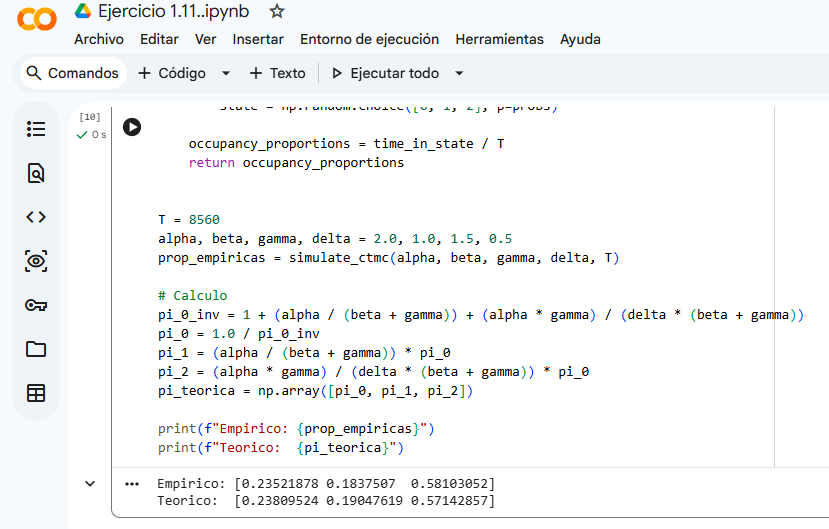
\includegraphics[width=0.5\textwidth]{../../Archivos/LOGOS_IMG/py110.PNG}
    \caption{Ejercicio 1.10. Ver en: \url{https://colab.research.google.com/drive/16v98OYc6ZjK0dpyIj9MJ-3UWCJs_UBRp?usp=sharing}}
    \label{python110}
\end{figure}

\textbf{c Discusión de la convergencia ergódica:}
    A medida que aumentamos el valor del 
    horizonte temporal $T$, observaremos 
    (por la Ley Fuerte de los Grandes 
    Números para Cadenas de Markov, 
    probada en el Ejercicio 1.6) que las
     proporciones empíricas 
     $\frac{1}{T}\int_0^T \mathbf{1}_{\{X_s=i\}} ds$ convergen casi 
     seguramente al vector probabilístico 
     estacionario $\pi$. Para valores de $T$ 
     pequeños, la varianza de la trayectoria 
     hace que la distribución empírica 
     varíe considerablemente dependiendo del 
     estado inicial $X_0$; sin embargo, para 
     $T$ suficientemente grande 
     (ej. $T \ge 10^4/\max(|A_{ii}|)$), el 
     sistema olvida su condición inicial y 
     pasa una fracción de tiempo en cada 
     estado exactamente proporcional a la medida invariante $\pi$.
\end{proof}



\begin{ejercicio}{Simulación en Python: nacimiento-muerte con deriva}{1.12}
    Considere la cadena nacimiento-muerte sobre $\mathbb{N}_0$ con $\lambda_n \equiv \lambda$ y $\mu_n \equiv \mu \mathbf{1}_{\{n\ge 1\}}$. Simule para $\lambda < \mu$, $\lambda = \mu$ y $\lambda > \mu$. Analice cualitativamente, estime la media temporal y explique cómo el experimento distingue los regímenes.
\end{ejercicio}


\newpage

\begin{proof}[Solución Ejercicio 1.12]
\textbf{Implementación en Python (Simulación y cálculo de la media empírica):}
\begin{lstlisting}[language=Python, basicstyle=\footnotesize\ttfamily, frame=single, numbers=left]
import numpy as np
import matplotlib.pyplot as plt

def simulate_birth_death(lam, mu, T, initial_state=0):
    t = 0.0
    state = initial_state
    
    times = [t]
    states = [state]
    integral_X = 0.0 # Para calcular la media empirica
    
    while t < T:
        rate_up = lam
        rate_down = mu if state > 0 else 0.0
        total_rate = rate_up + rate_down
        
        holding_time = np.random.exponential(1.0 / total_rate)
        
        # Area bajo la curva = estado * tiempo transcurrido en el estado
        actual_time = min(holding_time, T - t)
        integral_X += state * actual_time
        
        t += holding_time
        if t >= T: break
            
        # Determinar direccion del salto
        if np.random.rand() < (rate_up / total_rate):
            state += 1
        else:
            state -= 1
            
        times.append(t)
        states.append(state)
        
    times.append(T)
    states.append(states[-1])
    
    mean_X = integral_X / T
    return np.array(times), np.array(states), mean_X

# Parametros para regimen subcritico (recurrente positivo)
lam_sub, mu_sub, T = 4.0, 5.0, 1000.0
t_sub, X_sub, mean_emp_sub = simulate_birth_death(lam_sub, mu_sub, T)

# Media Teorica M/M/1
rho = lam_sub / mu_sub
mean_teo_sub = rho / (1 - rho)
print(f"Media empirica: {mean_emp_sub:.4f}, Media Teorica: {mean_teo_sub:.4f}")
\end{lstlisting}

\begin{figure}[h]
    \centering
    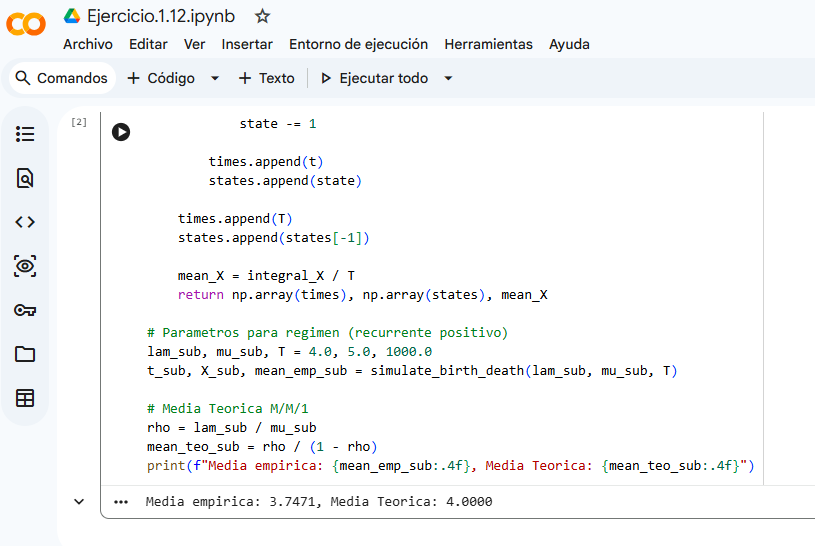
\includegraphics[width=0.5\textwidth]{../../Archivos/LOGOS_IMG/py112.PNG}
    \caption{Ejercicio 1.12. Ver en: \url{https://colab.research.google.com/drive/1YP99EH_K0xuzFXvZAhbW3jwVzzqCZnWX?usp=sharing}}
    \label{python112}
\end{figure}


    \textbf{b Análisis cualitativo de trayectorias:}
    \begin{itemize}
        \item \textbf{Subcrítico ($\lambda < \mu$):} La gráfica de $X_t$ muestra regresión a la media. La cadena sube pero es constantemente "empujada" hacia el 0. El sistema es estable y posee una distribución invariante geométrica.
        \item \textbf{Crítico ($\lambda = \mu$):} La gráfica muestra un comportamiento similar a un movimiento browniano o caminata aleatoria no sesgada. Presenta excursiones largas lejos del cero, pero eventualmente retorna. Es un sistema nulo recurrente; la varianza crece con el tiempo y no existe una media estacionaria finita.
        \item \textbf{Supercrítico ($\lambda > \mu$):} La gráfica muestra una clara pendiente positiva con tendencia lineal. El número de individuos crece indefinidamente hacia infinito. Es un sistema transiente.
    \end{itemize}

    \textbf{d Por qué el experimento distingue los regímenes:}
    El análisis empírico temporal ($\frac{1}{T}\int_0^T X_s ds$) se convierte en el estadístico decisivo.
    En el régimen recurrente positivo ($\lambda < \mu$), este estadístico converge rápidamente a un número constante y finito (la media teórica $\frac{\lambda}{\mu-\lambda}$). En el régimen crítico y supercrítico, si intentamos calcular esta integral empírica y la graficamos en función de $T$, veremos que el valor empírico no se estabiliza, sino que diverge hacia el infinito a medida que aumenta el tiempo de simulación, confirmando experimentalmente la ausencia de ergodicidad.
\end{proof}

\newpage

\section{Proceso de Poisson y sus extensiones elementales}
\subsection{Proceso de Poisson}

\begin{ejercicio}{Ley, PGF y CF}{2.1}
    Sea $(N_t)_{t\ge 0}$ un proceso de Poisson homogéneo de intensidad $\lambda > 0$. A partir de la propiedad de incrementos independientes y estacionarios, demuestre que
    \[ \mathbb{P}(N_t = n) = e^{-\lambda t}\frac{(\lambda t)^n}{n!}, \quad n \in \mathbb{N}_0. \]
    Obtenga además la función generadora de probabilidades y la función característica de $N_t$.
\end{ejercicio}

\begin{proof}[Solución 2.1]
    \textbf{Deducción de la distribución de Poisson:}
    Definamos $P_n(t) = \mathbb{P}(N_t = n)$. Por axiomas del proceso de Poisson, para un intervalo infinitesimal $h \downarrow 0$:
    \begin{align*}
        P_0(h) &= 1 - \lambda h + o(h) \\
        P_1(h) &= \lambda h + o(h) \\
        \sum_{n \ge 2} P_n(h) &= o(h)
    \end{align*}
    Usando la propiedad de incrementos independientes y estacionarios, calculamos la probabilidad de $0$ llegadas en $t+h$:
    \[ P_0(t+h) = \mathbb{P}(N_t=0)\mathbb{P}(N_{t+h}-N_t=0) = P_0(t)P_0(h) = P_0(t)(1 - \lambda h + o(h)). \]
    Reacomodando y tomando el límite cuando $h \to 0$:
    \[ P_0'(t) = \lim_{h \downarrow 0} \frac{P_0(t+h) - P_0(t)}{h} = -\lambda P_0(t). \]
    La solución a esta ecuación diferencial, con condición inicial $P_0(0) = 1$, es $P_0(t) = e^{-\lambda t}$.

    Para $n \ge 1$, el evento $\{N_{t+h} = n\}$ puede ocurrir de varias formas disjuntas:
    \begin{itemize}
        \item $n$ llegadas en $t$ y $0$ en $h$: $P_n(t)P_0(h)$
        \item $n-1$ llegadas en $t$ y $1$ en $h$: $P_{n-1}(t)P_1(h)$
        \item $n-k$ llegadas en $t$ y $k \ge 2$ en $h$: contribuye $o(h)$.
    \end{itemize}
    Por tanto, $P_n(t+h) = P_n(t)(1-\lambda h) + P_{n-1}(t)(\lambda h) + o(h)$.
    Tomando el límite, obtenemos un sistema de ecuaciones diferenciales lineales:
    \[ P_n'(t) = -\lambda P_n(t) + \lambda P_{n-1}(t). \]
    Multiplicando por el factor integrante $e^{\lambda t}$:
    \[ \frac{d}{dt} \left( e^{\lambda t} P_n(t) \right) = \lambda e^{\lambda t} P_{n-1}(t). \]
    Procedemos por inducción. Supongamos $P_{n-1}(t) = e^{-\lambda t} \frac{(\lambda t)^{n-1}}{(n-1)!}$. Sustituyendo:
    \[ \frac{d}{dt} \left( e^{\lambda t} P_n(t) \right) = \lambda \frac{(\lambda t)^{n-1}}{(n-1)!}. \]
    Integrando de $0$ a $t$ (notando que $P_n(0) = 0$ para $n \ge 1$):
    \[ e^{\lambda t} P_n(t) = \frac{\lambda^n t^n}{n!} \implies P_n(t) = e^{-\lambda t}\frac{(\lambda t)^n}{n!}. \]

    \textbf{2. Función Generadora de Probabilidades (PGF):}
    Sea $s \in \mathbb{R}$ con $|s| \le 1$. La PGF es $G(s) = \mathbb{E}[s^{N_t}]$:
    \[ G(s) = \sum_{n=0}^\infty s^n e^{-\lambda t} \frac{(\lambda t)^n}{n!} = e^{-\lambda t} \sum_{n=0}^\infty \frac{(s\lambda t)^n}{n!}. \]
    Reconociendo la serie de Taylor de la exponencial:
    \[ G(s) = e^{-\lambda t} e^{s\lambda t} = \exp\left(\lambda t (s-1)\right). \]

    \textbf{3. Función Característica (CF):}
    Para $u \in \mathbb{R}$, la CF es $\phi(u) = \mathbb{E}[e^{iuN_t}]$. Esto es evaluar la PGF en $s = e^{iu}$:
    \[ \phi(u) = G(e^{iu}) = \exp\left(\lambda t (e^{iu}-1)\right). \]
\end{proof}

\newpage
\subsection{Tiempos entre saltos}

\begin{ejercicio}{Tiempos entre saltos y Ley Gamma}{2.2}
    Sea $T_n := \inf\{t \ge 0 : N_t = n\}$ el tiempo del $n$-ésimo salto. Demuestre que los tiempos entre saltos $S_n := T_n - T_{n-1}$ son i.i.d. exponenciales de parámetro $\lambda$, y deduzca que $T_n$ tiene ley $\text{Gamma}(n, \lambda)$. Calcule $\mathbb{E}[T_n]$ y $\text{Var}(T_n)$.
\end{ejercicio}

\begin{proof}[Solución 2.2]
    \textbf{Tiempos entre saltos (i.i.d. Exponenciales):}
    Para el primer salto $S_1 = T_1$:
    \[ \mathbb{P}(S_1 > t) = \mathbb{P}(N_t = 0) = e^{-\lambda t}. \]
    Esto significa que $S_1 \sim \text{Exp}(\lambda)$.
    Para $S_n$ con $n > 1$, condicionamos sobre el instante del salto anterior $T_{n-1} = s$:
    \[ \mathbb{P}(S_n > t \mid T_{n-1} = s) = \mathbb{P}(N_{s+t} - N_s = 0 \mid N_s = n-1). \]
    Por la propiedad de incrementos independientes y estacionarios del proceso de Poisson, el incremento $N_{s+t} - N_s$ es independiente de la historia hasta el tiempo $s$ ($N_s = n-1$) y tiene la misma distribución que $N_t$:
    \[ \mathbb{P}(S_n > t \mid T_{n-1} = s) = \mathbb{P}(N_t = 0) = e^{-\lambda t}. \]
    Como la probabilidad condicional no depende de $s$ ni de $n$, concluimos que todos los $S_n$ son independientes e idénticamente distribuidos como $\text{Exp}(\lambda)$.

    \textbf{2. Ley de $T_n$:}
    Notemos que $T_n = S_1 + S_2 + \dots + S_n$. La suma de $n$ variables aleatorias i.i.d. exponenciales de parámetro $\lambda$ sigue una distribución Gamma con parámetro de forma $n$ y de tasa $\lambda$. Por lo tanto:
    \[ T_n \sim \text{Gamma}(n, \lambda), \quad \text{con densidad } f_{T_n}(t) = \frac{\lambda^n t^{n-1}}{(n-1)!}e^{-\lambda t}, \ t \ge 0. \]

    \textbf{3. Momentos de $T_n$:}
    Usando la linealidad de la esperanza y la independencia para la varianza:
    \[ \mathbb{E}[T_n] = \mathbb{E}\left[ \sum_{i=1}^n S_i \right] = \sum_{i=1}^n \mathbb{E}[S_i] = \sum_{i=1}^n \frac{1}{\lambda} = \frac{n}{\lambda}. \]
    \[ \text{Var}(T_n) = \text{Var}\left( \sum_{i=1}^n S_i \right) = \sum_{i=1}^n \text{Var}(S_i) = \sum_{i=1}^n \frac{1}{\lambda^2} = \frac{n}{\lambda^2}. \]
\end{proof}

\newpage
\subsection{Orden condicionados}

\begin{ejercicio}{Estadísticos de orden condicionados}{2.3}
    Condicionado a $\{N_t = n\}$, muestre que los tiempos de salto ordenados $0 < T_1 < \dots < T_n \le t$ se distribuyen como estadísticos de orden de $n$ variables i.i.d. uniformes en $[0, t]$. Interprete esto. Deduca una fórmula para $\mathbb{E}\left[ \sum_{k=1}^{N_t} h(T_k) \mid N_t = n \right]$.
\end{ejercicio}

\begin{proof}[Solución 2.3]
    \textbf{Distribución Condicional Conjunta:}
    Queremos encontrar la densidad conjunta condicional $f_{T_1,\dots,T_n \mid N_t=n}(t_1, \dots, t_n)$ para $0 < t_1 < t_2 < \dots < t_n \le t$.
    El evento $\{T_1 \in dt_1, \dots, T_n \in dt_n, N_t = n\}$ equivale a tener exactamente un salto en cada intervalo infinitesimal $[t_i, t_i+dt_i]$ y cero saltos en los demás subintervalos de $[0, t]$.
    Por independencia y estacionariedad:
    \begin{align*}
        \mathbb{P}(T_1 \in dt_1, \dots, T_n \in dt_n, N_t = n) &= \left( \prod_{i=1}^n \mathbb{P}(1 \text{ salto en } dt_i) \right) \mathbb{P}(0 \text{ saltos en el resto del tiempo}) \\
        &= (\lambda dt_1) \dots (\lambda dt_n) \cdot e^{-\lambda (t - dt_1 - \dots - dt_n)}.
    \end{align*}
    Ignorando los $dt_i$ en el exponencial, la densidad conjunta no condicional es $\lambda^n e^{-\lambda t}$ sobre el símplex $0 < t_1 < \dots < t_n \le t$.
    Aplicando el teorema de Bayes para condicionar:
    \[ f_{T_1,\dots,T_n \mid N_t=n}(t_1, \dots, t_n) = \frac{f_{T_1,\dots,T_n, N_t}(t_1, \dots, t_n, n)}{\mathbb{P}(N_t = n)} = \frac{\lambda^n e^{-\lambda t}}{e^{-\lambda t} \frac{(\lambda t)^n}{n!}} = \frac{n!}{t^n}. \]
    Reconocemos $\frac{n!}{t^n}$ exactamente como la función de densidad conjunta de los estadísticos de orden de $n$ variables aleatorias i.i.d. con distribución Uniforme en $[0, t]$ (ya que cada una tiene densidad $1/t$, su producto es $1/t^n$, y hay $n!$ permutaciones posibles).

    \textbf{Interpretación:}
    Si sabemos que llegaron exactamente $n$ clientes en la jornada $[0, t]$, los tiempos de llegada no tienen ninguna preferencia o "acumulación" en la mañana o en la tarde. Si perdiéramos el orden cronológico y "revolviéramos" los tickets de llegada en una urna, la distribución sería indistinguible de haber generado $n$ puntos completamente al azar (uniformes) a lo largo del intervalo $[0, t]$.

    \textbf{Deducción de la fórmula para funciones medibles:}
    Como $T_1, \dots, T_n$ condicionados a $N_t=n$ tienen la misma distribución que los estadísticos de orden $U_{(1)}, \dots, U_{(n)}$ de $n$ variables i.i.d. $U_i \sim \text{Unif}(0,t)$, y dado que la suma es invariante ante permutaciones:
    \[ \sum_{k=1}^n h(T_k) \stackrel{d}{=} \sum_{k=1}^n h(U_{(k)}) = \sum_{i=1}^n h(U_i). \]
    Tomando esperanza:
    \[ \mathbb{E}\left[ \sum_{k=1}^n h(T_k) \mid N_t = n \right] = \mathbb{E}\left[ \sum_{i=1}^n h(U_i) \right] = \sum_{i=1}^n \mathbb{E}[h(U_i)] = n \mathbb{E}[h(U_1)]. \]
    Sabiendo que $U_1 \sim \text{Unif}(0,t)$, calculamos la esperanza con su integral:
    \[ \mathbb{E}\left[ \sum_{k=1}^{N_t} h(T_k) \mid N_t = n \right] = \frac{n}{t} \int_0^t h(x) dx. \]
\end{proof}

\newpage

\subsection{Adelgazamiento de Poisson}

\begin{ejercicio}{Adelgazamiento de Poisson (Thinning)}{2.4}
    Sea $(N_t)_{t\ge 0}$ un proceso de Poisson de intensidad $\lambda$, y marque cada salto de manera independiente con probabilidad $p \in (0,1)$. Defina $N_t^{(1)}$ como el número de saltos marcados y $N_t^{(0)}$ como el número de saltos no marcados hasta tiempo $t$. Demuestre que $N^{(1)}$ y $N^{(0)}$ son procesos de Poisson independientes con intensidades $\lambda p$ y $\lambda(1-p)$.
\end{ejercicio}

\begin{proof}[Solución 2.4]
    Para probar que son procesos independientes con las distribuciones indicadas en un tiempo $t$ fijo, calcularemos la probabilidad conjunta $\mathbb{P}(N_t^{(1)} = n, N_t^{(0)} = m)$. 
    
    Notemos que el evento $\{N_t^{(1)} = n, N_t^{(0)} = m\}$ implica que el número total de saltos es $N_t = n + m$. Condicionamos sobre este número total:
    \begin{align*}
        \mathbb{P}(N_t^{(1)} = n, N_t^{(0)} = m) &= \mathbb{P}(N_t^{(1)} = n, N_t = n + m) \\
        &= \mathbb{P}(N_t^{(1)} = n \mid N_t = n + m) \mathbb{P}(N_t = n + m).
    \end{align*}
    Sabemos que $N_t \sim \text{Poisson}(\lambda t)$, por lo que $\mathbb{P}(N_t = n+m) = e^{-\lambda t} \frac{(\lambda t)^{n+m}}{(n+m)!}$.
    Dado que ocurrieron $n+m$ saltos y cada uno se marca independientemente con probabilidad $p$, el número de saltos marcados sigue una distribución Binomial con parámetros $n+m$ y $p$:
    \[ \mathbb{P}(N_t^{(1)} = n \mid N_t = n + m) = \binom{n+m}{n} p^n (1-p)^m = \frac{(n+m)!}{n! m!} p^n (1-p)^m. \]
    Sustituyendo ambas expresiones en la probabilidad conjunta y reacomodando términos:
    \begin{align*}
        \mathbb{P}(N_t^{(1)} = n, N_t^{(0)} = m) &= \left( \frac{(n+m)!}{n! m!} p^n (1-p)^m \right) \left( e^{-\lambda t} \frac{(\lambda t)^{n+m}}{(n+m)!} \right) \\
        &= \frac{1}{n! m!} p^n (1-p)^m e^{-\lambda p t} e^{-\lambda (1-p) t} (\lambda t)^n (\lambda t)^m \\
        &= \left( e^{-\lambda p t} \frac{(\lambda p t)^n}{n!} \right) \left( e^{-\lambda (1-p) t} \frac{(\lambda (1-p) t)^m}{m!} \right).
    \end{align*}
    El resultado se factoriza en el producto de dos funciones de masa de probabilidad de Poisson: una con parámetro $\lambda p t$ y otra con parámetro $\lambda(1-p)t$. 
    Esto demuestra dos cosas simultáneamente:
    1. Las distribuciones marginales son $N_t^{(1)} \sim \text{Poisson}(\lambda p t)$ y $N_t^{(0)} \sim \text{Poisson}(\lambda(1-p) t)$.
    2. Al factorizarse la probabilidad conjunta en el producto de sus marginales, las variables $N_t^{(1)}$ y $N_t^{(0)}$ son independientes.
    Dado que este procedimiento aplica de igual forma para los incrementos en cualquier intervalo $(s, t]$, se concluye que son procesos de Poisson independientes.
\end{proof}

\newpage

\subsection{Superposición de Poisson}

\begin{ejercicio}{Superposición de procesos de Poisson}{2.5}
    Sean $N^{(1)}, \dots, N^{(m)}$ procesos de Poisson independientes con intensidades $\lambda_1, \dots, \lambda_m$. Muestre que la suma $N_t := \sum_{j=1}^m N_t^{(j)}$ es un proceso de Poisson de intensidad $\lambda_1 + \dots + \lambda_m$. Pruebe además que, condicionado a un salto de $N$, la probabilidad de que provenga de $N^{(j)}$ es $\frac{\lambda_j}{\lambda_1 + \dots + \lambda_m}$.
\end{ejercicio}


\begin{proof}[Solución 2.5]
    \textbf{1. Distribución de la Suma (Vía Funciones Generadoras):}
    Sea $\Lambda = \sum_{j=1}^m \lambda_j$. Conocemos que la función generadora de probabilidades (PGF) para un proceso $N_t^{(j)} \sim \text{Poisson}(\lambda_j t)$ es $G_{N^{(j)}}(s) = \exp(\lambda_j t (s-1))$.
    Como los procesos son mutuamente independientes, la PGF de su suma es el producto de sus respectivas PGFs:
    \begin{align*}
        G_{N_t}(s) &= \mathbb{E}\left[s^{\sum_{j=1}^m N_t^{(j)}}\right] = \prod_{j=1}^m \mathbb{E}\left[s^{N_t^{(j)}}\right] \\
        &= \prod_{j=1}^m \exp(\lambda_j t (s-1)) = \exp\left( \sum_{j=1}^m \lambda_j t (s-1) \right) = \exp(\Lambda t (s-1)).
    \end{align*}
    Esta es exactamente la PGF de una distribución de Poisson con parámetro $\Lambda t$. Como los procesos originales tienen incrementos independientes y estacionarios, su suma heredará estas propiedades, demostrando que $N_t$ es un proceso de Poisson de intensidad $\Lambda$.

    \textbf{2. Probabilidad condicional del origen de un salto:}
    Consideremos un intervalo infinitesimal $[t, t+h]$. El evento "ocurre un salto en $N$" significa que la suma de los procesos tuvo un incremento de $1$, lo cual (salvo eventos de probabilidad $o(h)$) ocurre si exactamente uno de los $N^{(k)}$ tiene un salto y los demás tienen cero.
    \begin{align*}
        \mathbb{P}(\text{salto es de } N^{(j)} \mid \text{salto en } N) &= \lim_{h \downarrow 0} \frac{\mathbb{P}(N_{t+h}^{(j)} - N_t^{(j)} = 1 \text{ y } N_{t+h}^{(k)} - N_t^{(k)} = 0 \text{ para } k \neq j)}{\mathbb{P}(N_{t+h} - N_t = 1)} \\
        &= \lim_{h \downarrow 0} \frac{ (\lambda_j h e^{-\lambda_j h}) \prod_{k \neq j} (e^{-\lambda_k h}) }{ \Lambda h e^{-\Lambda h} } \\
        &= \lim_{h \downarrow 0} \frac{\lambda_j h e^{-\Lambda h}}{\Lambda h e^{-\Lambda h}} = \frac{\lambda_j}{\Lambda} = \frac{\lambda_j}{\lambda_1 + \dots + \lambda_m}.
    \end{align*}
\end{proof}

\newpage

\subsection{Proceso de Poisson Compuesto}

\begin{ejercicio}{Proceso de Poisson Compuesto (Siniestros agregados)}{2.6}
    Sea $N_t$ un proceso de Poisson de intensidad $\lambda$ e $(Y_n)_{n\ge 1}$ una sucesión i.i.d. independiente de $N$, con $\mathbb{E}[|Y_1|] < \infty$. Defina $X_t := \sum_{k=1}^{N_t} Y_k$. Calcule $\mathbb{E}[X_t]$, $\text{Var}(X_t)$ y la función característica de $X_t$. Explique el significado.
\end{ejercicio}

\begin{proof}[Solución 2.6]
    \textbf{1. Esperanza (Ley de Esperanza Total / Identidad de Wald):}
    Condicionamos sobre el número de siniestros $N_t$:
    \[ \mathbb{E}[X_t] = \mathbb{E}[\mathbb{E}[X_t \mid N_t]] = \mathbb{E}\left[ \mathbb{E}\left[ \sum_{k=1}^{N_t} Y_k \mid N_t \right] \right]. \]
    Dado $N_t = n$, la suma tiene $n$ términos i.i.d., por lo que la esperanza interna es $n \mathbb{E}[Y_1]$:
    \[ \mathbb{E}[X_t] = \mathbb{E}[ N_t \mathbb{E}[Y_1] ] = \mathbb{E}[Y_1] \mathbb{E}[N_t] = \lambda t \mathbb{E}[Y_1]. \]

    \textbf{2. Varianza (Ley de Varianza Total):}
    Usamos la fórmula $\text{Var}(X_t) = \mathbb{E}[\text{Var}(X_t \mid N_t)] + \text{Var}(\mathbb{E}[X_t \mid N_t])$.
    \begin{align*}
        \text{Var}(X_t \mid N_t = n) &= \text{Var}\left(\sum_{k=1}^n Y_k\right) = n\text{Var}(Y_1) \implies \mathbb{E}[\text{Var}(X_t \mid N_t)] = \mathbb{E}[N_t \text{Var}(Y_1)] = \lambda t \text{Var}(Y_1). \\
        \mathbb{E}[X_t \mid N_t = n] &= n\mathbb{E}[Y_1] \implies \text{Var}(\mathbb{E}[X_t \mid N_t]) = \text{Var}(N_t \mathbb{E}[Y_1]) = (\mathbb{E}[Y_1])^2 \text{Var}(N_t) = \lambda t (\mathbb{E}[Y_1])^2.
    \end{align*}
    Sumando ambas partes:
    \[ \text{Var}(X_t) = \lambda t \text{Var}(Y_1) + \lambda t (\mathbb{E}[Y_1])^2 = \lambda t (\text{Var}(Y_1) + (\mathbb{E}[Y_1])^2). \]
    Recordando que $\text{Var}(Y) = \mathbb{E}[Y^2] - (\mathbb{E}[Y])^2$, tenemos:
    \[ \text{Var}(X_t) = \lambda t \mathbb{E}[Y_1^2]. \]

    \textbf{3. Función Característica (CF):}
    La CF de $X_t$ es $\phi_{X_t}(u) = \mathbb{E}[e^{iuX_t}]$. Condicionamos nuevamente sobre $N_t$:
    \[ \phi_{X_t}(u) = \mathbb{E}\left[ \mathbb{E}\left[ \exp\left(iu \sum_{k=1}^{N_t} Y_k \right) \mid N_t \right] \right]. \]
    Dado $N_t = n$, por independencia de las $Y_k$, la esperanza de su suma exponencial es el producto de sus CFs individuales $\phi_Y(u)$:
    \[ \phi_{X_t}(u) = \mathbb{E}\left[ (\phi_{Y_1}(u))^{N_t} \right]. \]
    Esto equivale a evaluar la PGF de $N_t$ (que es $G_N(s) = \exp(\lambda t(s-1))$) en $s = \phi_{Y_1}(u)$:
    \[ \phi_{X_t}(u) = \exp\left( \lambda t (\phi_{Y_1}(u) - 1) \right). \]

    \textbf{Interpretación}
    El modelo separa la incertidumbre en dos fuentes: la \textit{frecuencia} de los siniestros (cuántos ocurren, regido por $\lambda$) y la \textit{severidad} de los mismos (cuánto cuesta cada uno, regido por $Y_1$). 
    La esperanza del costo agregado $\lambda t \mathbb{E}[Y_1]$ es simplemente la frecuencia esperada multiplicada por el costo medio por siniestro (prima pura).
    La varianza agregada $\lambda t \mathbb{E}[Y_1^2]$ es elegante porque demuestra que la volatilidad total depende no solo de la varianza del costo individual $\text{Var}(Y_1)$, sino también de su valor medio (el término adicional proviene de la incertidumbre pura de \textit{cuántos} reclamos llegarán).
\end{proof}

\newpage
\subsection{Proceso de Poisson CTMC}

\begin{ejercicio}{El proceso de Poisson como CTMC}{2.7}
    Muestre que el proceso de Poisson es una CTMC sobre $\mathbb{N}_0$ con generador $\alpha(n,n+1) = \lambda$ y $\alpha(n,n) = -\lambda$. Verifique $Lf(n) = \lambda(f(n+1)-f(n))$, obtenga las ecuaciones de Kolmogorov y recupere la ley de Poisson.
\end{ejercicio}

\begin{proof}[Solución 2.7]
    \textbf{1. Generador $L$:}
    La definición del operador generador aplicado a una función $f$ (pensándolo como el producto matriz-vector $Af$) es:
    \[ (Lf)(n) = \sum_{m=0}^\infty A(n,m)f(m). \]
    Como las únicas tasas no nulas desde $n$ son hacia $n+1$ (con tasa $\lambda$) y la diagonal (con tasa $-\lambda$ por ser conservativa), tenemos:
    \[ (Lf)(n) = A(n,n)f(n) + A(n,n+1)f(n+1) = -\lambda f(n) + \lambda f(n+1) = \lambda(f(n+1) - f(n)). \]

    \textbf{2. Ecuaciones de Kolmogorov Hacia Adelante (Forward):}
    Las probabilidades de transición $p_j(t) := \mathbb{P}(X_t=j \mid X_0=0)$ satisfacen la ecuación diferencial matricial $P'(t) = P(t)A$. 
    Fijando el estado inicial en $0$, la ecuación para el estado $j$ (donde condicionamos al último salto hacia $j$) es:
    \[ p'_j(t) = \sum_{k} p_k(t)A(k,j). \]
    El estado $j$ solo puede ser alcanzado desde $j-1$ (con tasa $\lambda$) y "abandonado" a tasa $\lambda$ (término diagonal $A(j,j)$).
    Por tanto, para $j \ge 1$:
    \[ p'_j(t) = \lambda p_{j-1}(t) - \lambda p_j(t). \]
    Para el estado frontera $j=0$, no hay estados previos que puedan llegar a él:
    \[ p'_0(t) = -\lambda p_0(t). \]

    \textbf{3. Resolución para la Ley de Poisson:}
    La ecuación para $j=0$ es una EDO lineal de primer orden separable. Con la condición inicial $p_0(0) = 1$:
    \[ \frac{dp_0(t)}{dt} = -\lambda p_0(t) \implies \int \frac{1}{p_0} dp_0 = \int -\lambda dt \implies \ln(p_0(t)) = -\lambda t \implies p_0(t) = e^{-\lambda t}. \]
    Para $j \ge 1$, reescribimos la ecuación diferencial y aplicamos el factor integrante $e^{\lambda t}$:
    \[ p'_j(t) + \lambda p_j(t) = \lambda p_{j-1}(t) \]
    \[ e^{\lambda t} p'_j(t) + \lambda e^{\lambda t} p_j(t) = \lambda e^{\lambda t} p_{j-1}(t) \implies \frac{d}{dt} \left( e^{\lambda t} p_j(t) \right) = \lambda e^{\lambda t} p_{j-1}(t). \]
    Procedemos por inducción, sabiendo que para $j=0$, $p_0(t) = e^{-\lambda t}$. Supongamos cierto para $j-1$ que $p_{j-1}(t) = e^{-\lambda t} \frac{(\lambda t)^{j-1}}{(j-1)!}$:
    \[ \frac{d}{dt} \left( e^{\lambda t} p_j(t) \right) = \lambda e^{\lambda t} \left( e^{-\lambda t} \frac{(\lambda t)^{j-1}}{(j-1)!} \right) = \lambda \frac{(\lambda t)^{j-1}}{(j-1)!}. \]
    Integrando ambos lados desde $0$ a $t$, recordando que la condición inicial es $p_j(0) = 0$ para $j \ge 1$:
    \[ e^{\lambda t} p_j(t) - 0 = \frac{\lambda^j t^j}{j!} \implies p_j(t) = e^{-\lambda t} \frac{(\lambda t)^j}{j!}. \]
    Hemos recuperado exactamente la función de masa de probabilidad de la distribución de Poisson, demostrando que el proceso de saltos simples es equivalente a la formulación matricial continua.
\end{proof}

\newpage

\subsection{Martingala}

\begin{ejercicio}{Martingala compensada y exponencial}{2.8}
    Sea $(N_t)_{t\ge 0}$ un proceso de Poisson de intensidad $\lambda$. Defina $M_t := N_t - \lambda t$.
    Pruebe que $(M_t)_{t\ge 0}$ es una martingala respecto de la filtración natural. Después, para cada $\theta \in \mathbb{R}$, pruebe que
    \[ Z_t^{(\theta)} := \exp\left( \theta N_t - \lambda t(e^\theta - 1) \right) \]
    es una martingala positiva. Interprete esta familia como martingalas exponenciales asociadas al compensador del proceso.
\end{ejercicio}

\begin{proof}[Solución 2.8]
    \textbf{1. $(M_t)_{t\ge 0}$ es una martingala:}
    Debemos verificar tres condiciones para $M_t$ con respecto a su filtración natural $\mathcal{F}_t = \sigma(N_s : s \le t)$:
    \begin{itemize}
        \item \textit{Adaptabilidad:} $M_t$ es $\mathcal{F}_t$-medible ya que $N_t$ lo es y $\lambda t$ es determinista.
        \item \textit{Integrabilidad:} $\mathbb{E}[|M_t|] \le \mathbb{E}[N_t] + \lambda t = \lambda t + \lambda t = 2\lambda t < \infty$.
        \item \textit{Propiedad de Martingala:} Para $0 \le s < t$:
        \begin{align*}
            \mathbb{E}[M_t \mid \mathcal{F}_s] &= \mathbb{E}[N_t - \lambda t \mid \mathcal{F}_s] \\
            &= \mathbb{E}[(N_t - N_s) + N_s - \lambda t \mid \mathcal{F}_s].
        \end{align*}
        Como $N_s$ es $\mathcal{F}_s$-medible, sale de la esperanza condicional. Como el incremento $N_t - N_s$ es independiente de $\mathcal{F}_s$ y se distribuye como $\text{Poisson}(\lambda(t-s))$, su esperanza condicional es igual a su esperanza incondicional:
        \begin{align*}
            \mathbb{E}[M_t \mid \mathcal{F}_s] &= \mathbb{E}[N_t - N_s] + N_s - \lambda t \\
            &= \lambda(t-s) + N_s - \lambda t \\
            &= N_s - \lambda s = M_s.
        \end{align*}
    \end{itemize}
    Por tanto, $M_t$ es una martingala.

    \textbf{2. $(Z_t^{(\theta)})_{t\ge 0}$ es una martingala positiva:}
    Es trivialmente positiva porque es la exponencial de una variable real. Es adaptable e integrable (ya que la función generadora de momentos de un Poisson es finita para todo $\theta$). 
    Verificamos la propiedad de martingala para $s < t$:
    \begin{align*}
        \mathbb{E}[Z_t^{(\theta)} \mid \mathcal{F}_s] &= \mathbb{E}\left[ \exp\left( \theta N_t - \lambda t(e^\theta - 1) \right) \mid \mathcal{F}_s \right] \\
        &= \mathbb{E}\left[ \exp\left( \theta(N_t - N_s) + \theta N_s - \lambda t(e^\theta - 1) \right) \mid \mathcal{F}_s \right].
    \end{align*}
    Factorizando los términos que son $\mathcal{F}_s$-medibles o deterministas:
    \begin{align*}
        \mathbb{E}[Z_t^{(\theta)} \mid \mathcal{F}_s] &= \exp\left( \theta N_s - \lambda t(e^\theta - 1) \right) \mathbb{E}\left[ \exp\left( \theta(N_t - N_s) \right) \mid \mathcal{F}_s \right].
    \end{align*}
    Usando la independencia de los incrementos y la función generadora de momentos del proceso de Poisson $\mathbb{E}[e^{\theta X}] = \exp(\mu(e^\theta - 1))$ donde $\mu = \lambda(t-s)$:
    \begin{align*}
        \mathbb{E}[Z_t^{(\theta)} \mid \mathcal{F}_s] &= \exp\left( \theta N_s - \lambda t(e^\theta - 1) \right) \exp\left( \lambda(t-s)(e^\theta - 1) \right) \\
        &= \exp\left( \theta N_s - \lambda t(e^\theta - 1) + \lambda t(e^\theta - 1) - \lambda s(e^\theta - 1) \right) \\
        &= \exp\left( \theta N_s - \lambda s(e^\theta - 1) \right) = Z_s^{(\theta)}.
    \end{align*}

    \textbf{3. Interpretación:}
    El proceso $N_t$ es una submartingala creciente. Por la descomposición de Doob-Meyer, se puede expresar como una martingala más un proceso creciente predecible (su compensador). Aquí, $\lambda t$ es exactamente el compensador determinista que "corrige" la tendencia ascendente de $N_t$ para hacer que $N_t - \lambda t$ sea justo ("fair game"). 
    La familia $Z_t^{(\theta)}$ representa las martingalas exponenciales asociadas (o de Doléans-Dade generalizadas) que son fundamentales para aplicar cambios de medida mediante el Teorema de Girsanov para procesos de saltos.
\end{proof}

\newpage
\subsection{markoviana del proceso de Poisson}

\begin{ejercicio}{Versión fuerte markoviana del proceso de Poisson}{2.9}
    Sea $(N_t)_{t\ge 0}$ un proceso de Poisson de intensidad $\lambda$ y defina el tiempo de primer salto $T_1 := \inf\{t > 0 : N_t = 1\}$. Muestre directamente, a partir de la propiedad sin memoria del tiempo exponencial, que el proceso desplazado $\tilde{N}_t := N_{T_1+t} - N_{T_1}$ es independiente de $\mathcal{F}_{T_1}$ y tiene la misma ley que $N$.
\end{ejercicio}

\begin{proof}[Solución 2.9]
    Sabemos por el Ejercicio 2.2 que los tiempos de inter-llegada $S_n := T_n - T_{n-1}$ (con $T_0 = 0$) son variables aleatorias i.i.d. con distribución $\text{Exp}(\lambda)$.
    El tiempo del primer salto es exactamente $T_1 = S_1$. 
    
    El proceso desplazado $\tilde{N}_t$ cuenta el número de eventos que ocurren estrictamente después de $T_1$ en una ventana de tamaño $t$. Los tiempos entre estos nuevos eventos son exactamente la sucesión $S_2, S_3, S_4, \dots$.
    
    La $\sigma$-álgebra $\mathcal{F}_{T_1}$ contiene toda la información del proceso hasta el instante $T_1$, lo cual, en esencia, solo es el valor del propio $T_1$ (es decir, $S_1$).
    
    Como la sucesión original de inter-llegadas $(S_n)_{n \ge 1}$ es i.i.d., la subsucesión $(S_2, S_3, \dots)$ es mutuamente independiente de $S_1$.
    Por lo tanto, la dinámica del proceso $\tilde{N}_t$ depende exclusivamente de $(S_2, S_3, \dots)$, lo que hace a $\tilde{N}_t$ probabilísticamente independiente de $\mathcal{F}_{T_1}$.
    
    Además, dado que las variables $(S_2, S_3, \dots)$ son i.i.d. $\text{Exp}(\lambda)$, son estadísticamente indistinguibles de la sucesión original $(S_1, S_2, \dots)$. Un proceso de conteo definido por inter-llegadas i.i.d. exponenciales de parámetro $\lambda$ es, por definición, un proceso de Poisson de intensidad $\lambda$. 
    
    \textbf{Interpretación:}
    Este resultado demuestra la \textbf{Propiedad Fuerte de Markov} para el proceso de Poisson. No solo los incrementos desde tiempos deterministas $t$ son independientes del pasado, sino que el proceso también "olvida" su historia y se reinicia idénticamente a sí mismo a partir de tiempos aleatorios significativos, conocidos como tiempos de paro (como $T_1$).
\end{proof}

\newpage
\subsection{Llamadas clasificadas}

\begin{ejercicio}{Llamadas clasificadas por tipo (Generalización de Adelgazamiento)}{2.10}
    A una central telefónica llegan llamadas según un proceso de Poisson de intensidad $\lambda$. Cada llamada es clasificada, de manera independiente, como consulta, queja o venta con probabilidades $p_1, p_2, p_3$ (con $p_1+p_2+p_3=1$). Demuestre que $(N^{(1)}, N^{(2)}, N^{(3)})$ tiene componentes Poisson independientes con intensidades $\lambda p_1, \lambda p_2, \lambda p_3$. Calcule además la probabilidad de que en $[0, t]$ haya al menos una llamada de cada tipo.
\end{ejercicio}

\begin{proof}[Solución 2.10]
    \textbf{1. Independencia y Ley Poisson de las componentes:}
    Este es el análogo en dimensión 3 del Ejercicio 2.4 (Thinning). Evaluaremos la probabilidad conjunta en un tiempo $t$.
    El evento $\{N_t^{(1)}=n_1, N_t^{(2)}=n_2, N_t^{(3)}=n_3\}$ implica que el número total de llamadas fue $N_t = n_1+n_2+n_3$.
    Condicionando sobre el total de llamadas:
    \[ \mathbb{P}(N_t^{(1)}=n_1, N_t^{(2)}=n_2, N_t^{(3)}=n_3) = \mathbb{P}(N_t^{(1)}=n_1, N_t^{(2)}=n_2, N_t^{(3)}=n_3 \mid N_t = n_1+n_2+n_3) \mathbb{P}(N_t = n_1+n_2+n_3). \]
    La primera probabilidad condicional, al clasificar independientemente cada llamada en una de tres categorías, sigue una distribución Multinomial:
    \[ \mathbb{P}(\text{clasificación} \mid N_t = n) = \frac{(n_1+n_2+n_3)!}{n_1! n_2! n_3!} p_1^{n_1} p_2^{n_2} p_3^{n_3}. \]
    La probabilidad marginal del proceso original es la de una Poisson:
    \[ \mathbb{P}(N_t = n_1+n_2+n_3) = e^{-\lambda t} \frac{(\lambda t)^{n_1+n_2+n_3}}{(n_1+n_2+n_3)!}. \]
    Multiplicando ambas expresiones, los factoriales $(n_1+n_2+n_3)!$ se cancelan. Usando que $e^{-\lambda t} = e^{-\lambda (p_1+p_2+p_3) t} = e^{-\lambda p_1 t} e^{-\lambda p_2 t} e^{-\lambda p_3 t}$:
    \begin{align*}
        \mathbb{P}(N_t^{(1)}=n_1, N_t^{(2)}=n_2, N_t^{(3)}=n_3) &= \frac{1}{n_1! n_2! n_3!} p_1^{n_1} p_2^{n_2} p_3^{n_3} e^{-\lambda p_1 t} e^{-\lambda p_2 t} e^{-\lambda p_3 t} (\lambda t)^{n_1} (\lambda t)^{n_2} (\lambda t)^{n_3} \\
        &= \left( e^{-\lambda p_1 t} \frac{(\lambda p_1 t)^{n_1}}{n_1!} \right) \left( e^{-\lambda p_2 t} \frac{(\lambda p_2 t)^{n_2}}{n_2!} \right) \left( e^{-\lambda p_3 t} \frac{(\lambda p_3 t)^{n_3}}{n_3!} \right).
    \end{align*}
    La función de probabilidad conjunta se factoriza exactamente en el producto de tres funciones de masa de Poisson individuales. Esto demuestra rigurosamente que $N^{(1)}_t, N^{(2)}_t$ y $N^{(3)}_t$ son variables aleatorias independientes para cada $t$, y que se distribuyen como procesos de Poisson con las intensidades especificadas $\lambda p_i$.

    \textbf{2. Probabilidad de al menos una llamada de cada tipo:}
    Sea el evento $E_i = \{N_t^{(i)} \ge 1\}$ (que es el complemento de tener cero llamadas de ese tipo).
    Dado que las tres componentes son procesos estocásticos independientes, la probabilidad de la intersección es el producto de las probabilidades individuales:
    \begin{align*}
        \mathbb{P}(E_1 \cap E_2 \cap E_3) &= \mathbb{P}(N_t^{(1)} \ge 1) \mathbb{P}(N_t^{(2)} \ge 1) \mathbb{P}(N_t^{(3)} \ge 1) \\
        &= \left( 1 - \mathbb{P}(N_t^{(1)} = 0) \right) \left( 1 - \mathbb{P}(N_t^{(2)} = 0) \right) \left( 1 - \mathbb{P}(N_t^{(3)} = 0) \right) \\
        &= \left( 1 - e^{-\lambda p_1 t} \right) \left( 1 - e^{-\lambda p_2 t} \right) \left( 1 - e^{-\lambda p_3 t} \right).
    \end{align*}
\end{proof}

\newpage
\subsection{Simulación en Python}

\begin{ejercicio}{Tiempos de salto y ley Gamma}{2.11}
    Sea $(N_t)$ un proceso de Poisson de intensidad $\lambda$.
    a. Genere en Python una gran muestra de tiempos entre saltos i.i.d. exponenciales y construya a partir de ellos los tiempos $T_n$ del $n$-ésimo salto.
    b. Para un $n$ fijo, compare mediante histogramas y superposición de densidades la distribución empírica de $T_n$ con la ley Gamma$(n, \lambda)$.
    c. Estime numéricamente $\mathbb{E}[T_n]$ y $\text{Var}(T_n)$ y compárelas con los valores exactos.
    d. Comente qué mejora al simular $T_n$ como suma de exponenciales en vez de reconstruirlo a partir de muchas trayectorias completas del conteo.
\end{ejercicio}

\begin{proof}[Solución 2.11]
    \textbf{Implementación en Python:}
    Utilizaremos NumPy para generar la matriz de tiempos entre saltos y SciPy para graficar la densidad teórica.

\begin{lstlisting}[language=Python, basicstyle=\footnotesize\ttfamily, frame=single, numbers=left]
import numpy as np
import matplotlib.pyplot as plt
import scipy.stats as stats

# Parametros
lam = 2.0  # Intensidad lambda
n = 5      # n-esimo salto
num_muestras = 100000

# Generacion de tiempos entre saltos S_i ~ Exp(lam)
# Numpy parametriza la exponencial con la escala (1/lambda)
S = np.random.exponential(scale=1.0/lam, size=(num_muestras, n))

# Construccion de T_n (Suma acumulada de S_i a lo largo de las filas)
T_n = np.sum(S, axis=1)

# Estimacion numerica de momentos
emp_mean = np.mean(T_n)
emp_var = np.var(T_n)

exact_mean = n / lam
exact_var = n / (lam**2)

print(f"Media - Empirica: {emp_mean:.4f} | Exacta: {exact_mean:.4f}")
print(f"Varianza - Empirica: {emp_var:.4f} | Exacta: {exact_var:.4f}")

# b Visualizacion: Histograma vs Densidad Teorica Gamma(n, lambda)
# Nota: scipy.stats.gamma usa 'a' como parametro de forma (n) y 'scale' como 1/lambda
x = np.linspace(0, np.max(T_n), 1000)
pdf_gamma = stats.gamma.pdf(x, a=n, scale=1.0/lam)

plt.figure(figsize=(8, 5))
plt.hist(T_n, bins=100, density=True, alpha=0.6, color='skyblue', label='Empirica (Histograma)')
plt.plot(x, pdf_gamma, 'r-', lw=2, label=f'Teorica Gamma({n}, {lam})')
plt.title(f'Distribucion del tiempo del salto $n={n}$')
plt.xlabel('Tiempo $T_n$')
plt.ylabel('Densidad')
plt.legend()
plt.grid(True, alpha=0.3)
plt.show()
\end{lstlisting}

\textbf{d Ventaja de simular como suma de exponenciales:}
    Si quisiéramos encontrar $T_n$ simulando la trayectoria completa de $N_t$, tendríamos que generar saltos iterativamente hasta que el contador llegue a $n$, o discretizar el tiempo en intervalos $\Delta t$ pequeñísimos y simular variables de Bernoulli, lo cual introduce un error de discretización sustancial y es computacionalmente ineficiente ($\mathcal{O}(T/\Delta t)$). 
    
    Al simular $T_n$ directamente como la suma de $n$ variables aleatorias exponenciales, la simulación es \textbf{exacta} (sin errores de discretización) y \textbf{óptima en tiempo} ($\mathcal{O}(n)$). Nos permite "saltar" inmediatamente a la información que necesitamos sin tener que trazar ni almacenar todo el historial del proceso $N_t$ paso por paso.
\end{proof}

\begin{figure}[h]
    \centering
    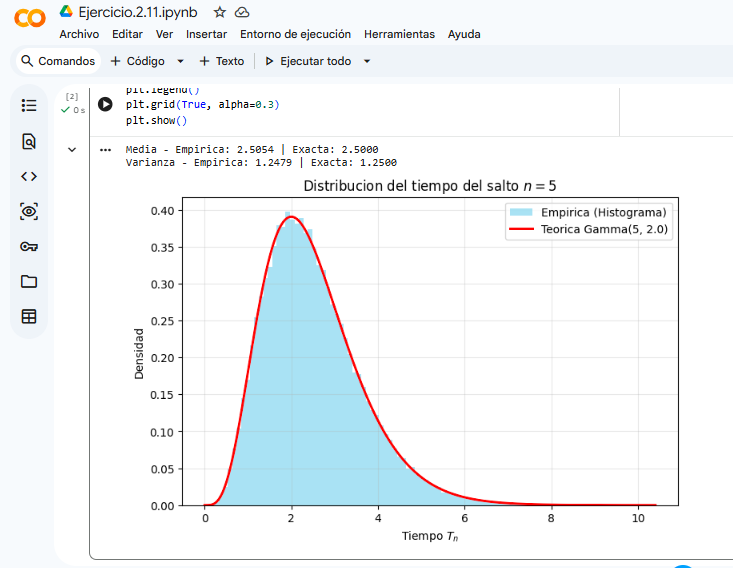
\includegraphics[width=0.5\textwidth]{../../Archivos/LOGOS_IMG/py211.PNG}
    \caption{Ejercicio 2.11. Ver en: \url{https://colab.research.google.com/drive/1MIGKtrn3AiP5yE1S4XLNVZ6_25cd2sZs?usp=sharing}}
    \label{python211}
\end{figure}


\newpage

\begin{ejercicio}{Simulación en Python: adelgazamiento y superposición}{2.12}
    Escriba un programa que simule un proceso de Poisson de intensidad $\lambda$ en $[0,T]$ y luego marque cada salto con probabilidad $p$.
    a. Verifique numéricamente que el proceso adelgazado tiene aproximadamente distribución Poisson$(\lambda p T)$.
    b. Estime la covarianza empírica entre los conteos del marcado y no marcado; compárela con la teórica.
    c. Simule dos Poisson independientes ($\lambda_1, \lambda_2$), súmelos y compare con Poisson$(\lambda_1 + \lambda_2)$.
    d. Discuta cómo ilustran la estructura algebraica de los procesos de Poisson.
\end{ejercicio}

\begin{proof}[Solución 2.12]
    \textbf{Implementación en Python :}
    Dado que solo nos interesa el número total de conteos en un tiempo fijo $T$ (y no los instantes exactos de tiempo), podemos muestrear directamente de la distribución de Poisson para hacer la simulación altamente eficiente.

\begin{lstlisting}[language=Python, basicstyle=\footnotesize\ttfamily, frame=single, numbers=left]
import numpy as np
import scipy.stats as stats

# Parametros generales
T = 10.0
num_muestras = 100000

print("--- ADELGAZAMIENTO (THINNING) ---")
lam = 5.0
p = 0.3

# Simulacion del proceso original en [0, T]
N_t_total = np.random.poisson(lam * T, num_muestras)

# Adelgazamiento: Dado N saltos, los marcados siguen una Binomial(N, p)
N_1 = np.random.binomial(N_t_total, p)
N_0 = N_t_total - N_1

# a) Verificacion de la distribucion del proceso marcado (N_1)
media_emp_N1 = np.mean(N_1)
var_emp_N1 = np.var(N_1)
param_teorico = lam * p * T

print(f"N_1 - Media Empirica: {media_emp_N1:.4f} | Teorica: {param_teorico:.4f}")
print(f"N_1 - Var Empirica:   {var_emp_N1:.4f} | Teorica: {param_teorico:.4f}")

# b) Covarianza entre marcados y no marcados
cov_matrix = np.cov(N_1, N_0)
cov_emp = cov_matrix[0, 1]
print(f"Covarianza empirica(N_1, N_0): {cov_emp:.4f} (Teorica: 0.0 debido a independencia)")

print("\n--- SUPERPOSICION ---")
lam1 = 3.0
lam2 = 4.0

# c) Simular independientes y sumar
N_A = np.random.poisson(lam1 * T, num_muestras)
N_B = np.random.poisson(lam2 * T, num_muestras)
N_sum = N_A + N_B

# Comparar con Poisson(lam1 + lam2)
media_emp_sum = np.mean(N_sum)
var_emp_sum = np.var(N_sum)
param_teorico_sum = (lam1 + lam2) * T

print(f"N_sum - Media Empirica: {media_emp_sum:.4f} | Teorica: {param_teorico_sum:.4f}")
print(f"N_sum - Var Empirica:   {var_emp_sum:.4f} | Teorica: {param_teorico_sum:.4f}")
\end{lstlisting}

    \textbf{Discusión sobre la estructura algebraica:}
    Las simulaciones ilustran numéricamente que los procesos de Poisson poseen una estructura algebraica, comportándose de manera isomorfa a la suma de vectores en un espacio lineal:
    \begin{itemize}
        \item \textbf{Descomposición (Thinning):} Actúa como un proyector ortogonal u operador de división. Si tomas un proceso padre y lo separas mediante lanzamientos de moneda independientes, no solo obtienes procesos Poisson hijos, sino que estos nacen completamente ortogonales (independientes) entre sí, como lo corrobora la covarianza empírica nula del inciso (b).
        \item \textbf{Adición (Superposición):} Actúa como un operador de suma. Si tienes varios procesos Poisson que operan en paralelo sin interferirse, al observarlos como un solo flujo agregado, el resultado no es un caos matemático, sino un nuevo proceso de Poisson cuya intensidad es la suma lineal exacta de las intensidades originales.
    \end{itemize}
    Estas propiedades permiten modelar redes de colas y flujos complejos (como datos en servidores o automóviles en una autopista) usando álgebra lineal simple sobre las intensidades.
\end{proof}

\begin{figure}[h]
    \centering
    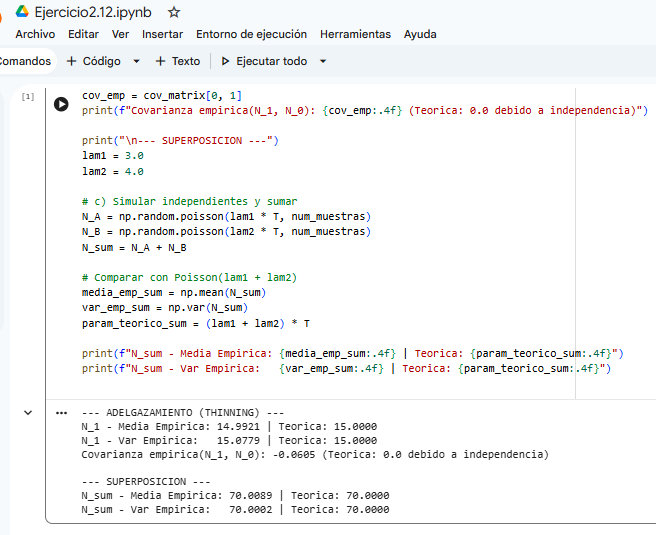
\includegraphics[width=0.5\textwidth]{../../Archivos/LOGOS_IMG/py212.PNG}
    \caption{Ejercicio 2.12. Ver en: \url{https://colab.research.google.com/drive/1i5YWB2JsKNRuH1unk3U1_OVEaMyRTOk-?usp=sharing}}
    \label{python212}
\end{figure}

\newpage

\section{Modelos de colas M/M/k y M/M/infinito}

\end{document}